\chapter{Capacitively Coupled Pixel Detectors for the CLIC Vertex Detector}
\label{chap:theory}

\chapterquote{There, sir! that is the perfection of vessels!}
{Jules Verne, 1828--1905}

%========================================================================================
%========================================================================================

\section{Introduction}
Identification of heavy-flavour quarks and tau-leptons relies upon precise reconstruction of the secondary displaced vertices produced in the decay of these particles as well as accurate association of daughter tracks to those vertices.  For the CLIC vertex detector very high spatial resolution, of approximately 3 {\mu}m, and good geometric coverage extending to low $\theta$ values are essential for achieving the precision on the reconstructed vertices necessary for identification of heavy-flavour quarks and tau-leptons.  The vertex detector must have a low material budget, less than 0.2 $\text{X}_{0}$ per layer, as to not impact the performance of the other sub detectors and have a low occupancy, which will be aided by time-tagging to an accuracy of 10 ns, to counter the high numbers of beam-induced background particles found near the impact point.  

As there are no commercially available technology options that fulfil all the criteria for the CLIC vertex detector, the CLIC experiment has developed a wide R\&D program in search for new technology options that could be used in the vertex detector.  High voltage complementary metal-oxide-semiconductor (HV-CMOS) active sensors coupled to a separate readout ASIC are one such option.  The performance of this option and the impact of mechanical tolerances that are present in the manufacturing process are presented.  

%========================================================================================

\subsection{Active Pixel Sensor, HV-CMOS}
There are two classifications for pixel detectors; hybrid detectors where a passive sensor is bump-bonded to a separate readout chip and fully integrated where a collection diode is built upon the same wafer as the readout circuitry.  Both of these technology options find the CLIC experimental conditions extremely challenging.  Hybrid technologies struggle to achieved both the radiation tolerance and the functionality in the readout circuitry, while fully integrated circuits typically have too slow readout times due to limitations on the bias voltage that can be applied.  

HV-CMOS is adapted to the CLIC experimental conditions as the n-MOS and p-MOS transistors forming the integrated amplifier (or generic in-pixel logic operations in general) for collecting the signal are embedded within a deep n-well, as shown in figure \ref{fig:hvcmos}.  This acts as both the collection diode as well as providing shielding to the circuitry from the beam induced radiation.  With the integrated circuitry shielded from the p-substrate it becomes possible to apply a large bias voltage to the substrate to widen the depletion region.  A wide depletion region causes more single charge to move via drift instead of diffusion, which provides the fast readout times required by the CLIC experiment.  

\begin{figure}
\centering
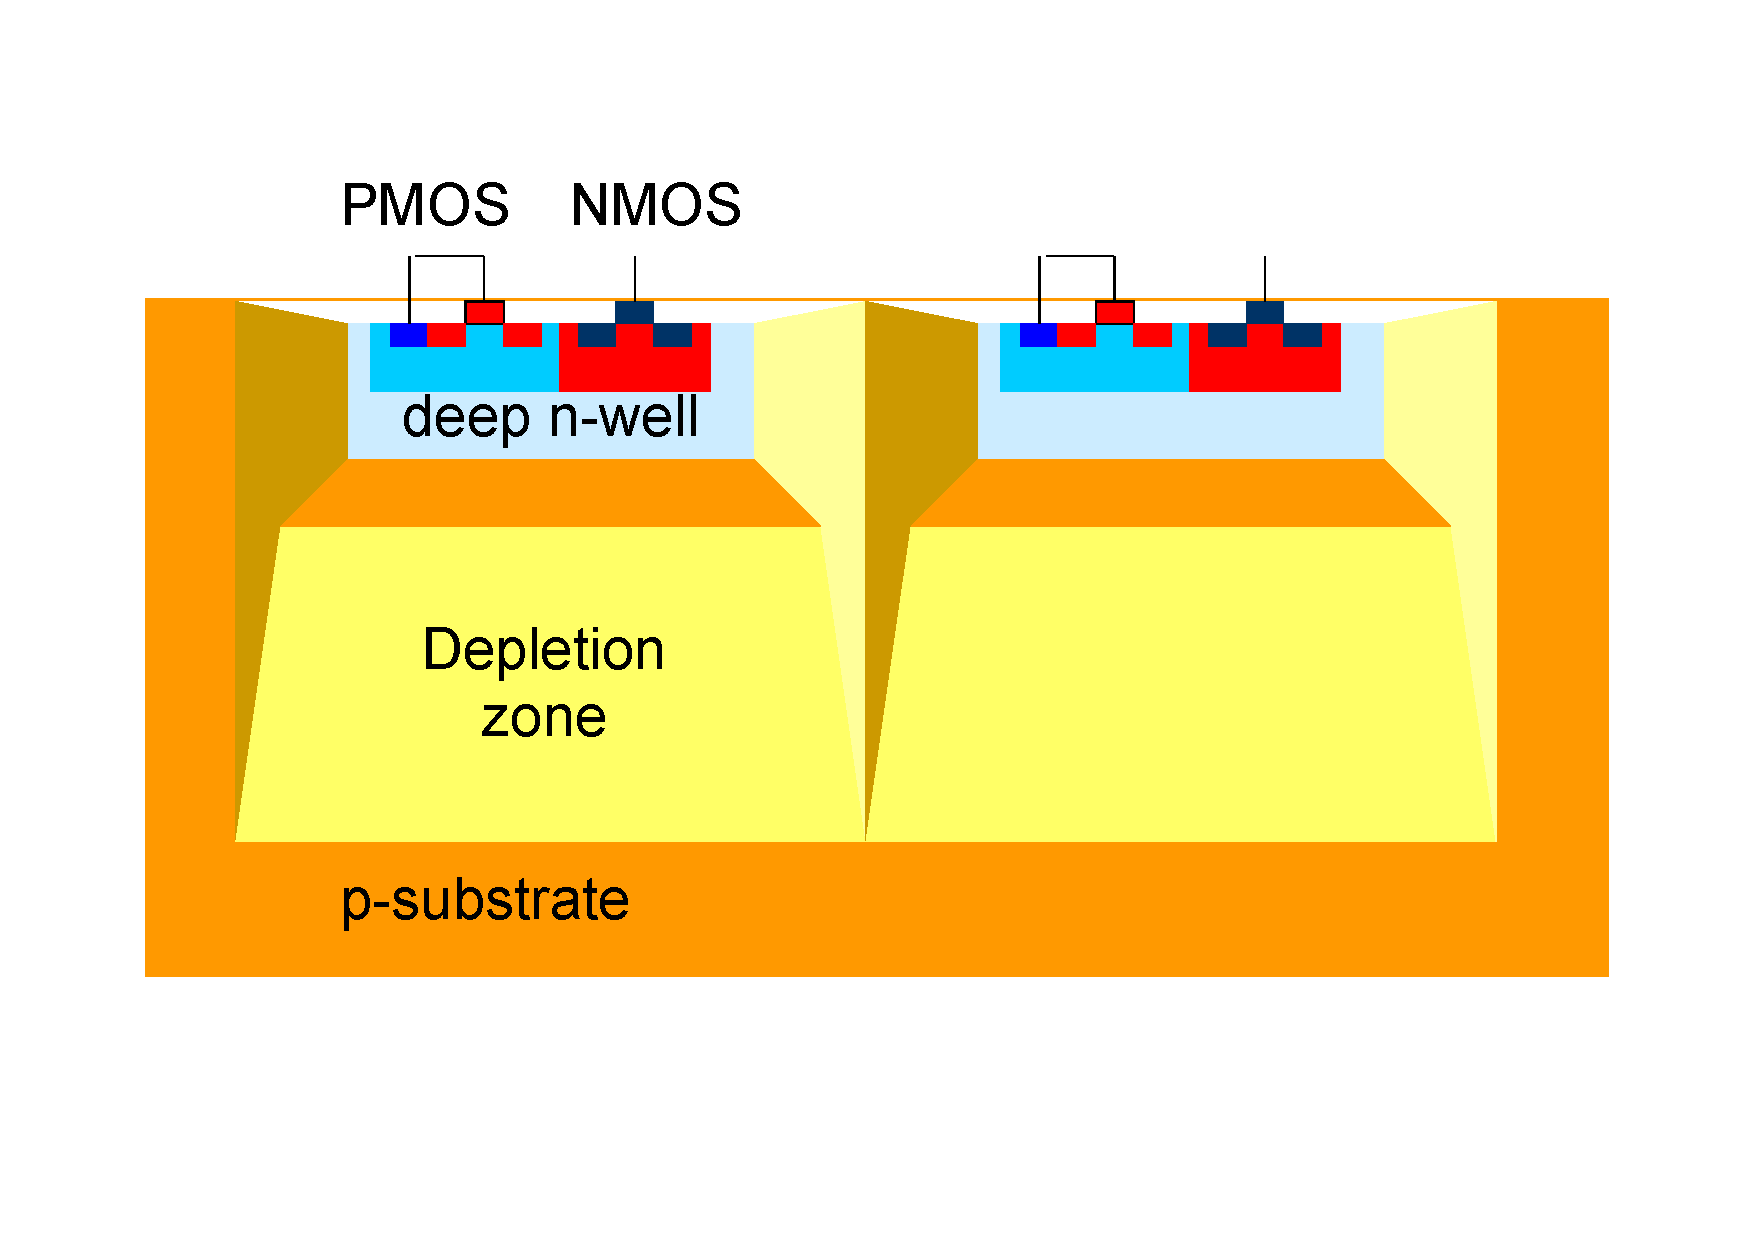
\includegraphics[width=0.75\textwidth]{CLICdpVertex/Plots/HV-CMOSDiagram.pdf}
\caption[HV-CMOS diagram.]{HV-CMOS diagram.}
\label{fig:hvcmos}
\end{figure}

HV-CMOS devices are strong candidates for the CLIC vertex detector, however, they do have limitations, such as noise from interference between the n and p doped wells of the n-MOS and p-MOS transistors that sit within the deep n well.  This noise will grow with the number of n-MOS and p-MOS devices on the wafer and so ultimately restricts the complexity of the in-pixel operations that can be performed.  Not only that, but the CMOS process cannot be trivially applied at all length scales, so manufacturing small sensors becomes increasingly more challenging.  Another drawback is the deep n well does not occupy the full space of the pixel, which means some signal charge can be lost in the sensor.  The CLIC conditions also induce drawbacks on the HV-CMOS performance as, to minimise the material budget, the sensor will be as thin as possible leading to a narrow depletion region and a small collected charge.  To counter this, in-pixel signal amplification was applied to the HV-CMOS devices, as shown in figure \ref{fig:ccpdandclicpix}.  This increases the signal going to the readout ASIC, which counteracts both the small collected charge and the intrinsically small capacitance between the HV-CMOS and readout ASIC.

\begin{figure}
\centering
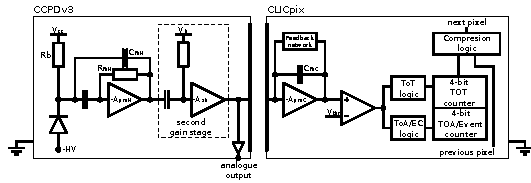
\includegraphics[width=1.0\textwidth]{CLICdpVertex/Plots/schematic.pdf}
\caption[Schematic of CCPDv3 and CLICpix pixels.]{Schematic of CCPDv3 and CLICpix pixels.}
\label{fig:ccpdandclicpix}
\end{figure}

%========================================================================================

\subsection{Readout ASIC, CLICpix}
The readout ASIC used in this study is the CLICpix, which is a charge integrating amplifier connected to a discriminator as shown in figure \ref{fig:ccpdandclicpix}.  The discriminator produces an output signal when the input signal is over a given threshold.  The discriminator output is then used as the input for further logic operations to record the magnitude, using a Time over Threshold (ToT) measurement, and time of arrival of the collected charge.  The ToT uses a four-bit readout and so is confined to the range 0 to 15 units.  It is envisaged that the CLICpix ASIC will be run using shutter-based operations where the entire matrix is kept active while the shutter is open and when closed the matrix is readout at once.  This would be appropriate for the CLIC experiment as it will run using pulses, containing bunches of $e^{+}$ and $e^{-}$, that are separated by 20 ms for readout time.  Each pulse contains 312 bunches, each bunch is 156 ns long and the bunch separation is 0.5 ns.  

Fluctuations will exist between individual pixels on the CLICpix sensor due to the manufacturing process, which if not accounted for would degrade the vertex detector performance.  To suppress these fluctuations, the CLICpix sensors have a 4-bit adjustment build into their front end that can be tuned on a per pixel basis to unify the response of the matrix.  The equalisation of the matrix response is achieved by first setting the four bits to 0000 for all pixels and then scanning over the input signal to the CLICpix, or DAC, to determine the point at which more than half the pixels are responding.  The same procedure is repeated using the 1111 setting to bound each pixels response.  By applying linear interpolation between the measurements of the half pixel turn on DAC value for these extreme bin adjustment settings it is possible to tune the response of each pixel.  Each pixel in the matrix is tuned to be as close as possible to the mean of all responses measured across the matrix in both the 0000 and 1111 settings.  

%========================================================================================

\subsection{Capacitive Coupling}
Solder bump-bonding is the typical method that is used for connecting active pixel sensors to the readout ASIC, however, the solder adds to the thickness of the sensor significantly and raises the cost.  A viable alternative to this involves using a thin uniform layer of glue to form a capacitive connection between the active pixel sensor and the readout ASIC.  While this procedure reduces cost and material budget for the sensor in comparison to bump-bonding, the gluing process introduces previously unseen complications that have to be considered.  

%========================================================================================

\section{Construction}
In the construction of pixel detectors that use a layer of glue to form a capacitive connection between the active pixel sensor and the readout ASIC it is possible to introduce misalignments between the sensor and ASIC.  The goal of this study it to categorise the effect such misalignments would have on the detector performance.  The sensitivity of the performance of the detector to these misalignments could determine whether capacitively coupled pixel detectors constructed in this way are a viable option for the CLIC vertex detector.  To quantify the impact of misalignments such as these a number of pixel detectors were constructed that contained misalignments between the HV-CMOS and CLICpix, as shown in figure \ref{fig:alignment}.  A table \ref{table:alignment} contains a summary of all the samples considered in this study.

\begin{figure}
\centering
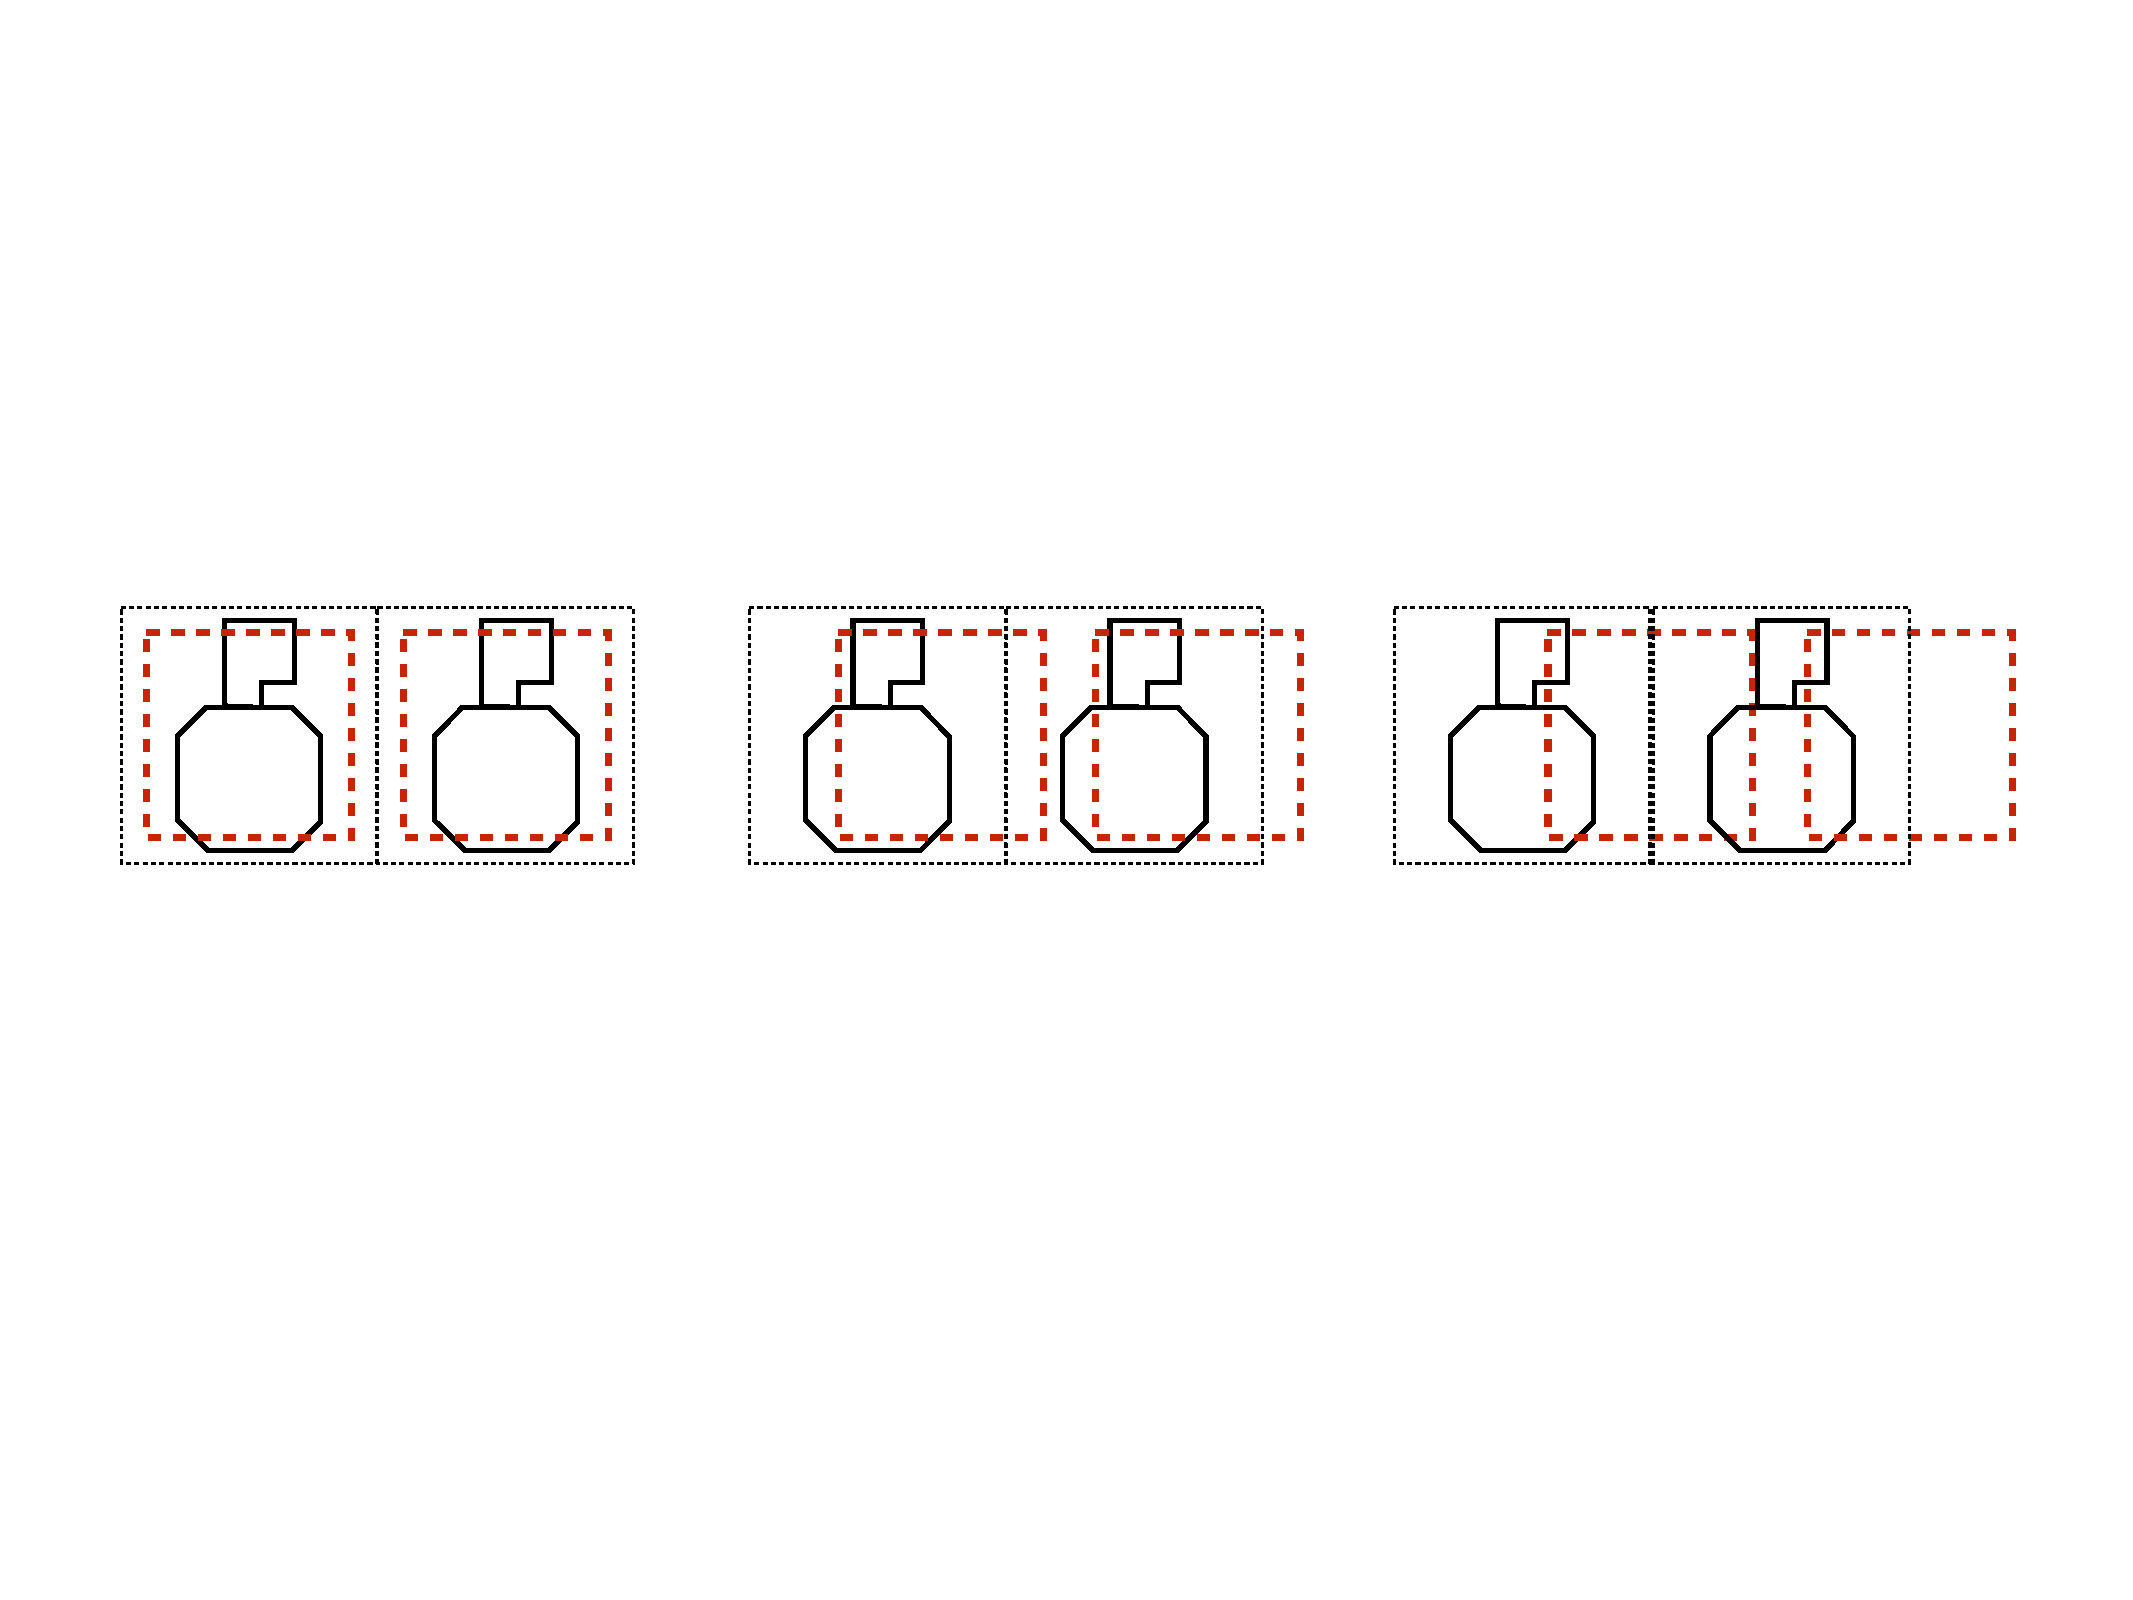
\includegraphics[width=1.0\textwidth]{CLICdpVertex/Plots/misalignedPads.pdf}
\caption[Schematic of alignment of CCPDv3 and CLICpix sensors studied in this analysis.]{Schematic of alignment of CCPDv3 and CLICpix sensors studied in this analysis.  The red dotted line represents the CCPDv3 and the solid black line represents the CLICpix.  From left to right; centred pixels, 1/4 offset (6.25 {\mu}m) and 1/2 offset (12.5 {\mu}m).}
\label{fig:alignment}
\end{figure}

\begin{table}[h!]
\centering
\begin{tabular}{ l l }
\hline
Assembly & Alignment \\ 
\hline
SET9 & Centred \\
SET10 & $\frac{1}{4}$ Offset \\
%SET11 & $\frac{1}{2}$ Offset \\
SET12 & Centred \\
SET13 & Centred \\
SET14 & $\frac{1}{2}$ Offset \\
SET15 & Centred \\
SET16 & $\frac{1}{2}$ Offset \\
\hline
\end{tabular}
\caption[A description of the alignment of the HV-CMOS active pixel sensor and the CLICpix readout ASIC for the pixel detectors considered in this study.]{A description of the alignment of the HV-CMOS active pixel sensor and the CLICpix readout ASIC for the pixel detectors considered in this study.}
\label{table:alignment}
\end{table}

The pitch of the sensors, both the HV-CMOS active pixel sensor and CLICpix readout ASIC, produced for this study was 25 {\mu}m and the matrix size was 64$\times$64.  The full details of the gluing process can be found here (CERN NOTE CITE) along with a study into the absolute precision of the manufacturing procedure.  It was found that for devices constructed in an identical fashion to those considered here, the glue layer thicknesses were less than 1 {\mu}m and the precision on the pixel positioning was less than 0.5 {\mu}m.  

%========================================================================================
%========================================================================================

\section{Device Characterisation}

%========================================================================================

\subsection{CLICPix Calibration}

\subsubsection{Experimental Setup}
In this experiment the CLICpix device was calibrated using a radioactive source, $\text{Sr}^{90}$, to generate the single in the active pixel sensor.  The unstable $\text{Sr}^{90}$ undergoes $\beta^{-}$ decay to form $\text{Y}^{90}$.  The $\text{Y}^{90}$, as it too is unstable, undergoes $\beta^{-}$ decay to form $\text{Z}^{90}$, which is stable.  Each $\beta^{-}$ decays produce an $\text{e}^{-}$ and a $\bar{\nu_{e}}$, and it is the $\text{e}^{-}$ that are used to generate the signal in the pixel detector.  The $\text{Sr}^{90}$ source used for this experiment had an activity of 29.6 MBq.  

This radioactive source was positioned directly on top of the pixel detector and measurements were made of both the ToT output from the CLICpix and the HV-CMOS analogue signal for individual pixels on the sensor.  The HV-CMOS pulse shape was recorded on a fast sampling oscilloscope that was also used to tigger the data taking for the CLICpix readout.  The on-pixel event counter was used to veto all events where multiple hits occurred within the time window for a given event.  

\begin{figure}
\centering
\subfloat[]{\label{fig:pulseshape1}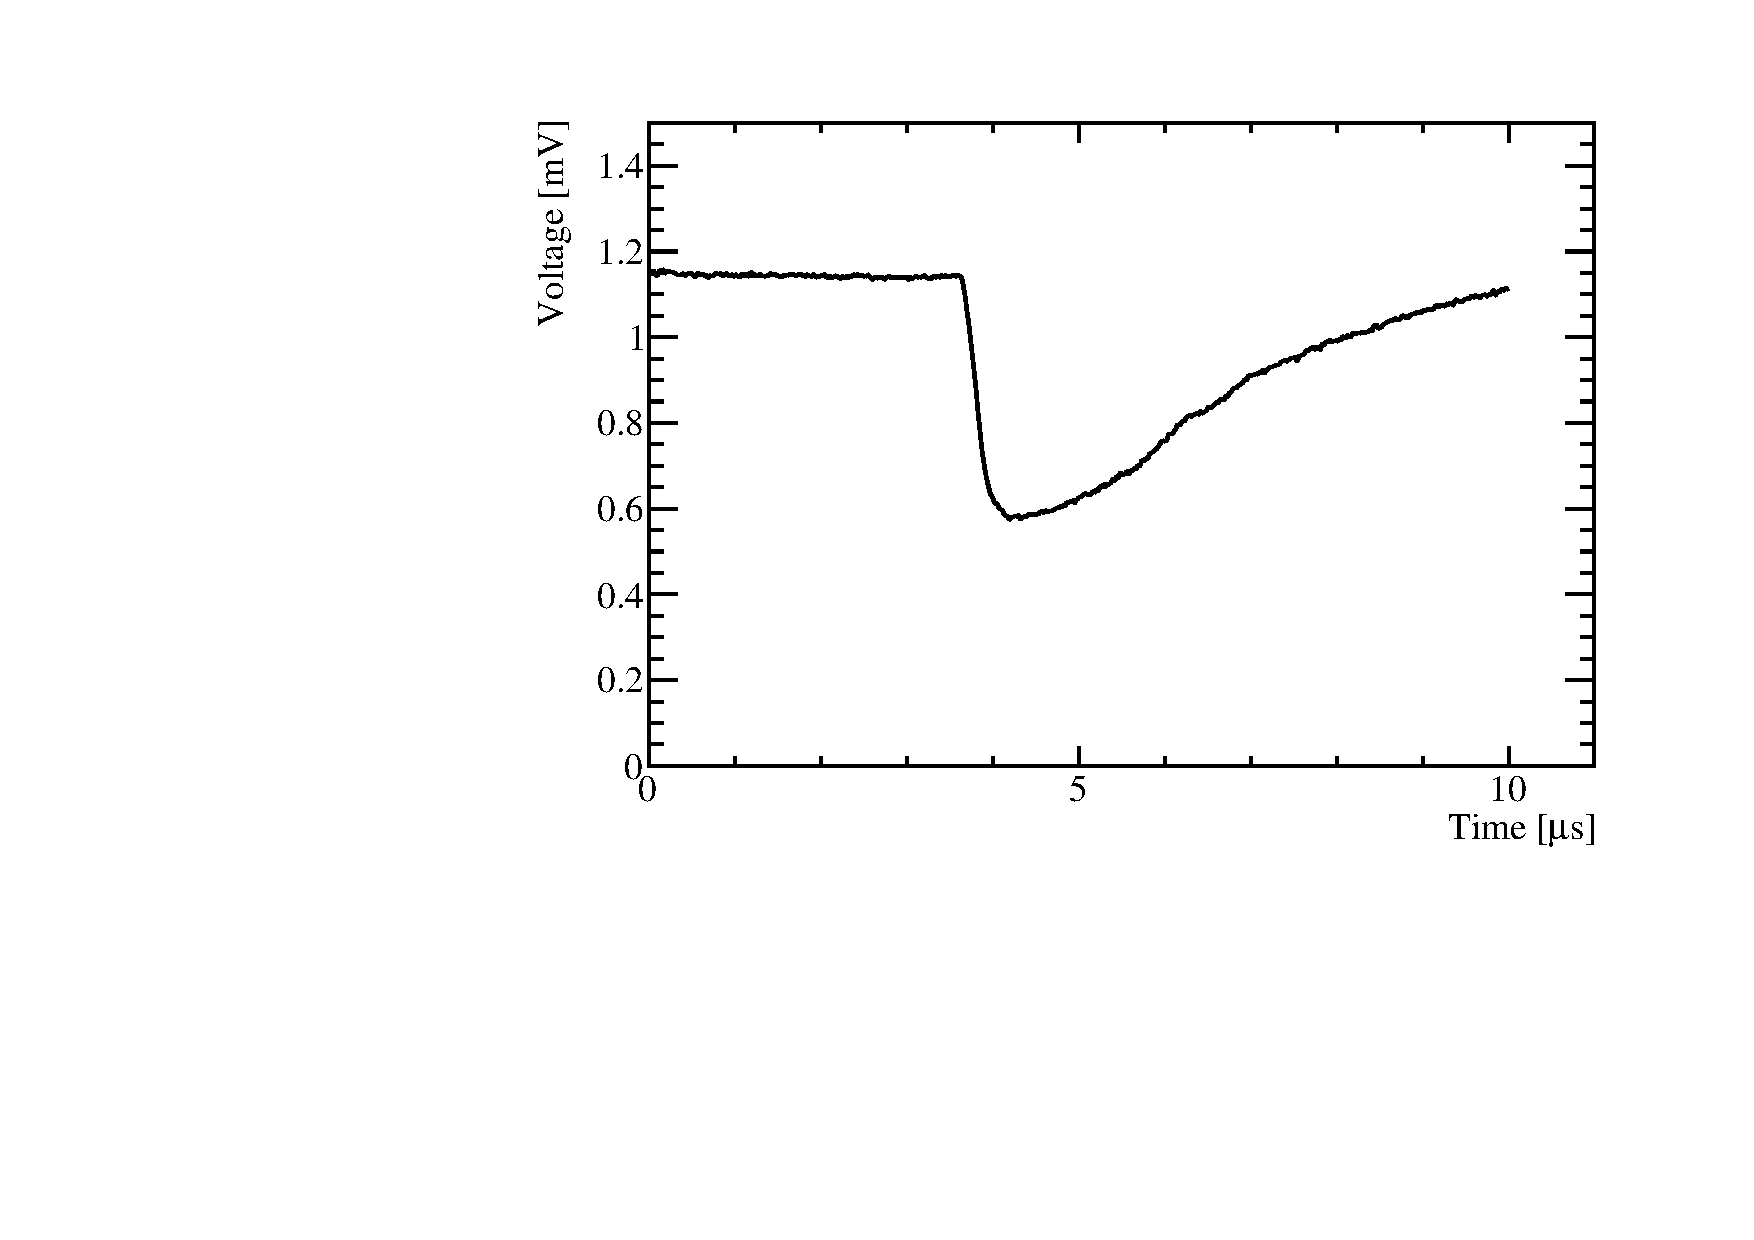
\includegraphics[width=0.5\textwidth]{CLICdpVertex/Plots/HV-CMOS/Frames/PulseShape01000NoOffset.pdf}}
\subfloat[]{\label{fig:pulseshape2}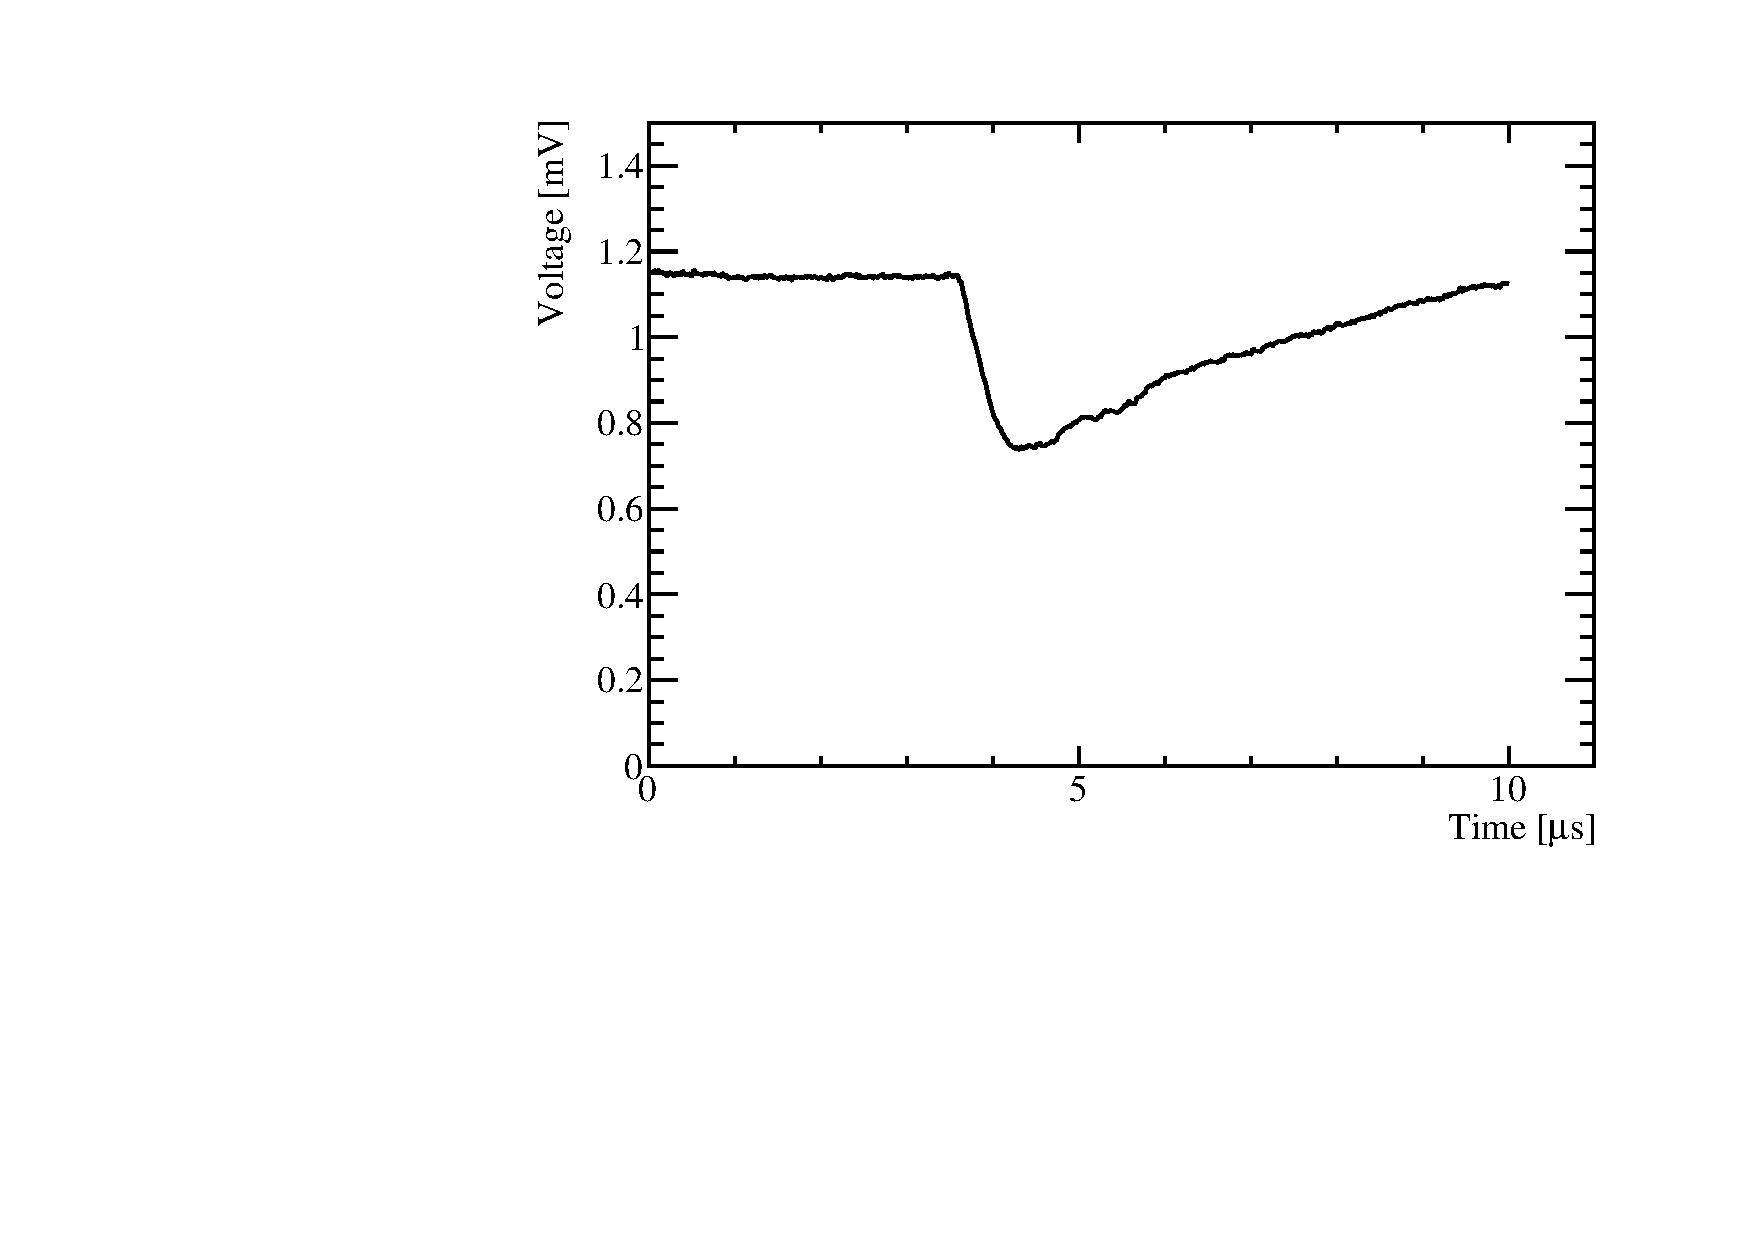
\includegraphics[width=0.5\textwidth]{CLICdpVertex/Plots/HV-CMOS/Frames/PulseShape01005NoOffset.pdf}}\hfill
\subfloat[]{\label{fig:pulseshape3}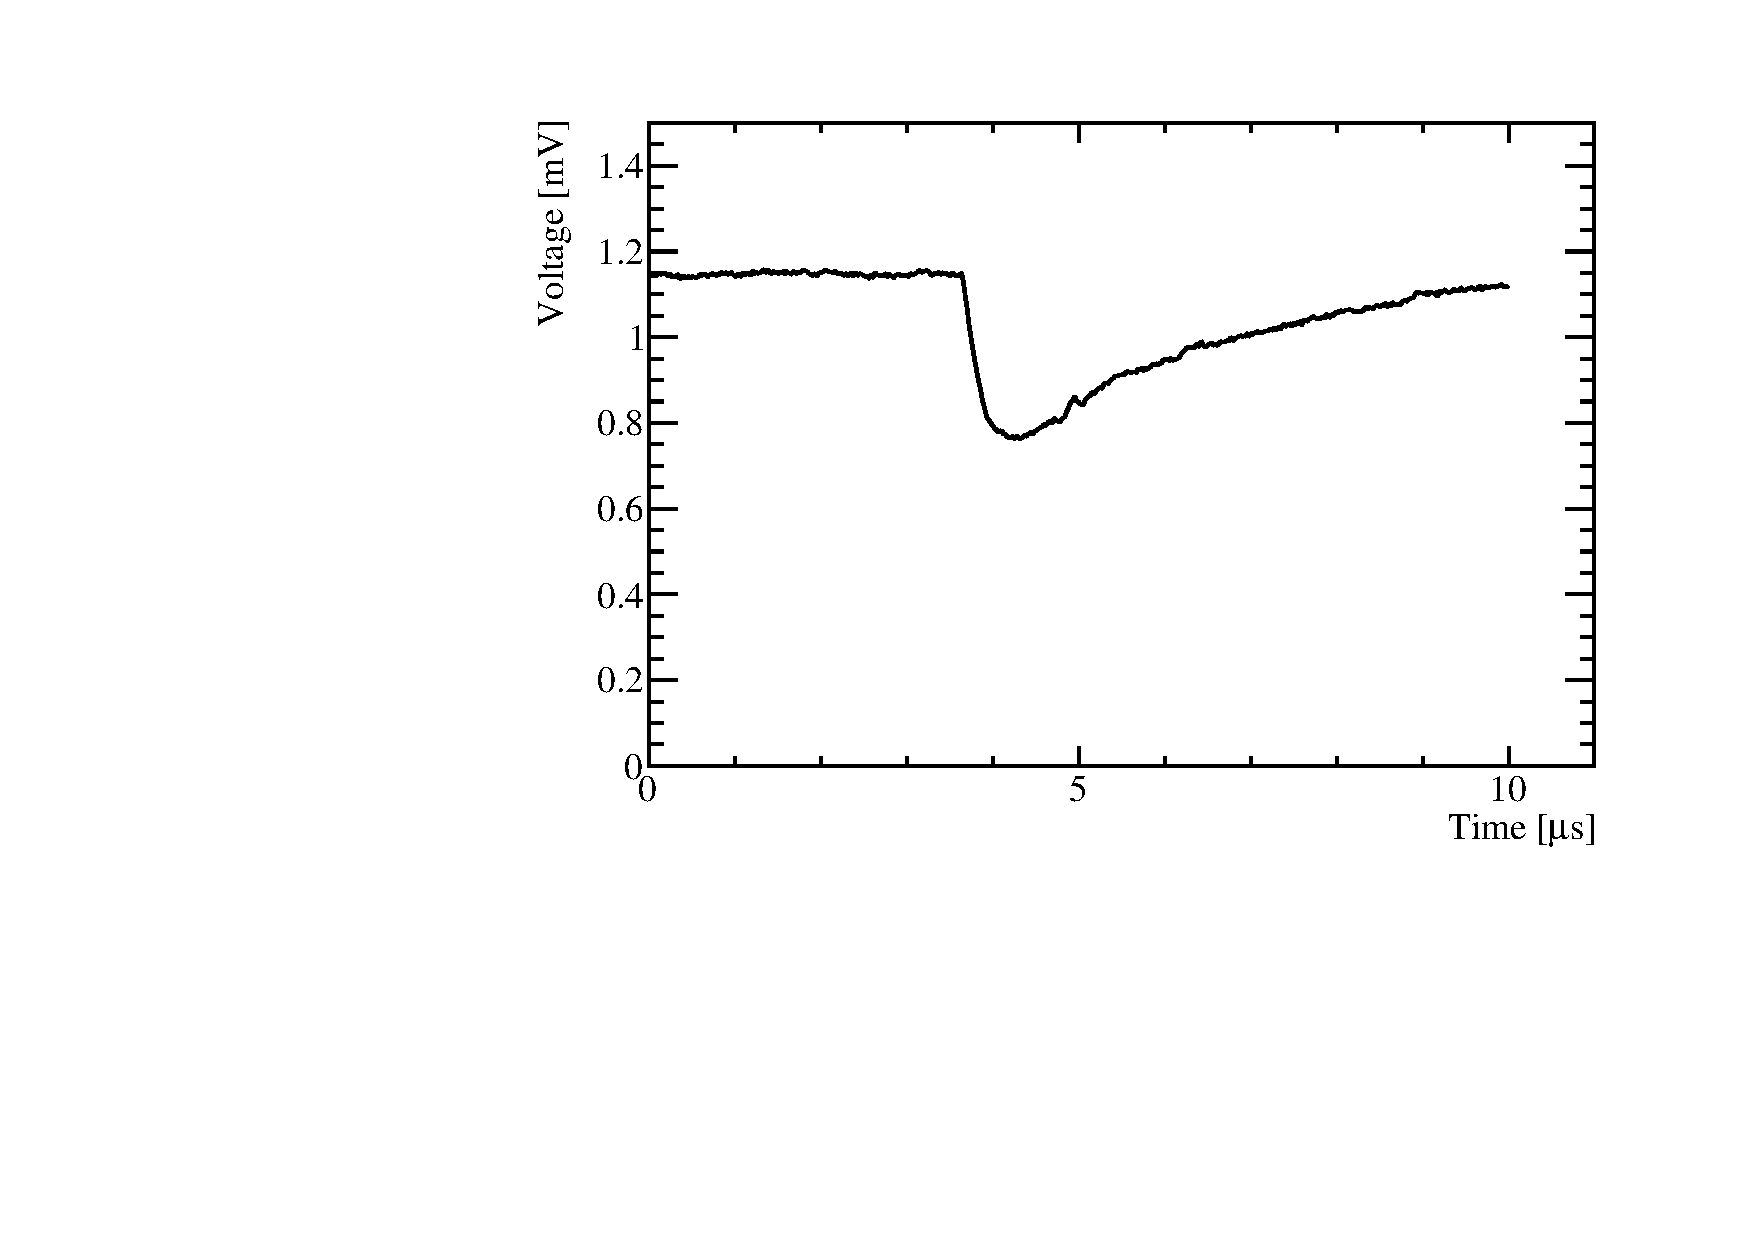
\includegraphics[width=0.5\textwidth]{CLICdpVertex/Plots/HV-CMOS/Frames/PulseShape01006NoOffset.pdf}}
\subfloat[]{\label{fig:pulseshape4}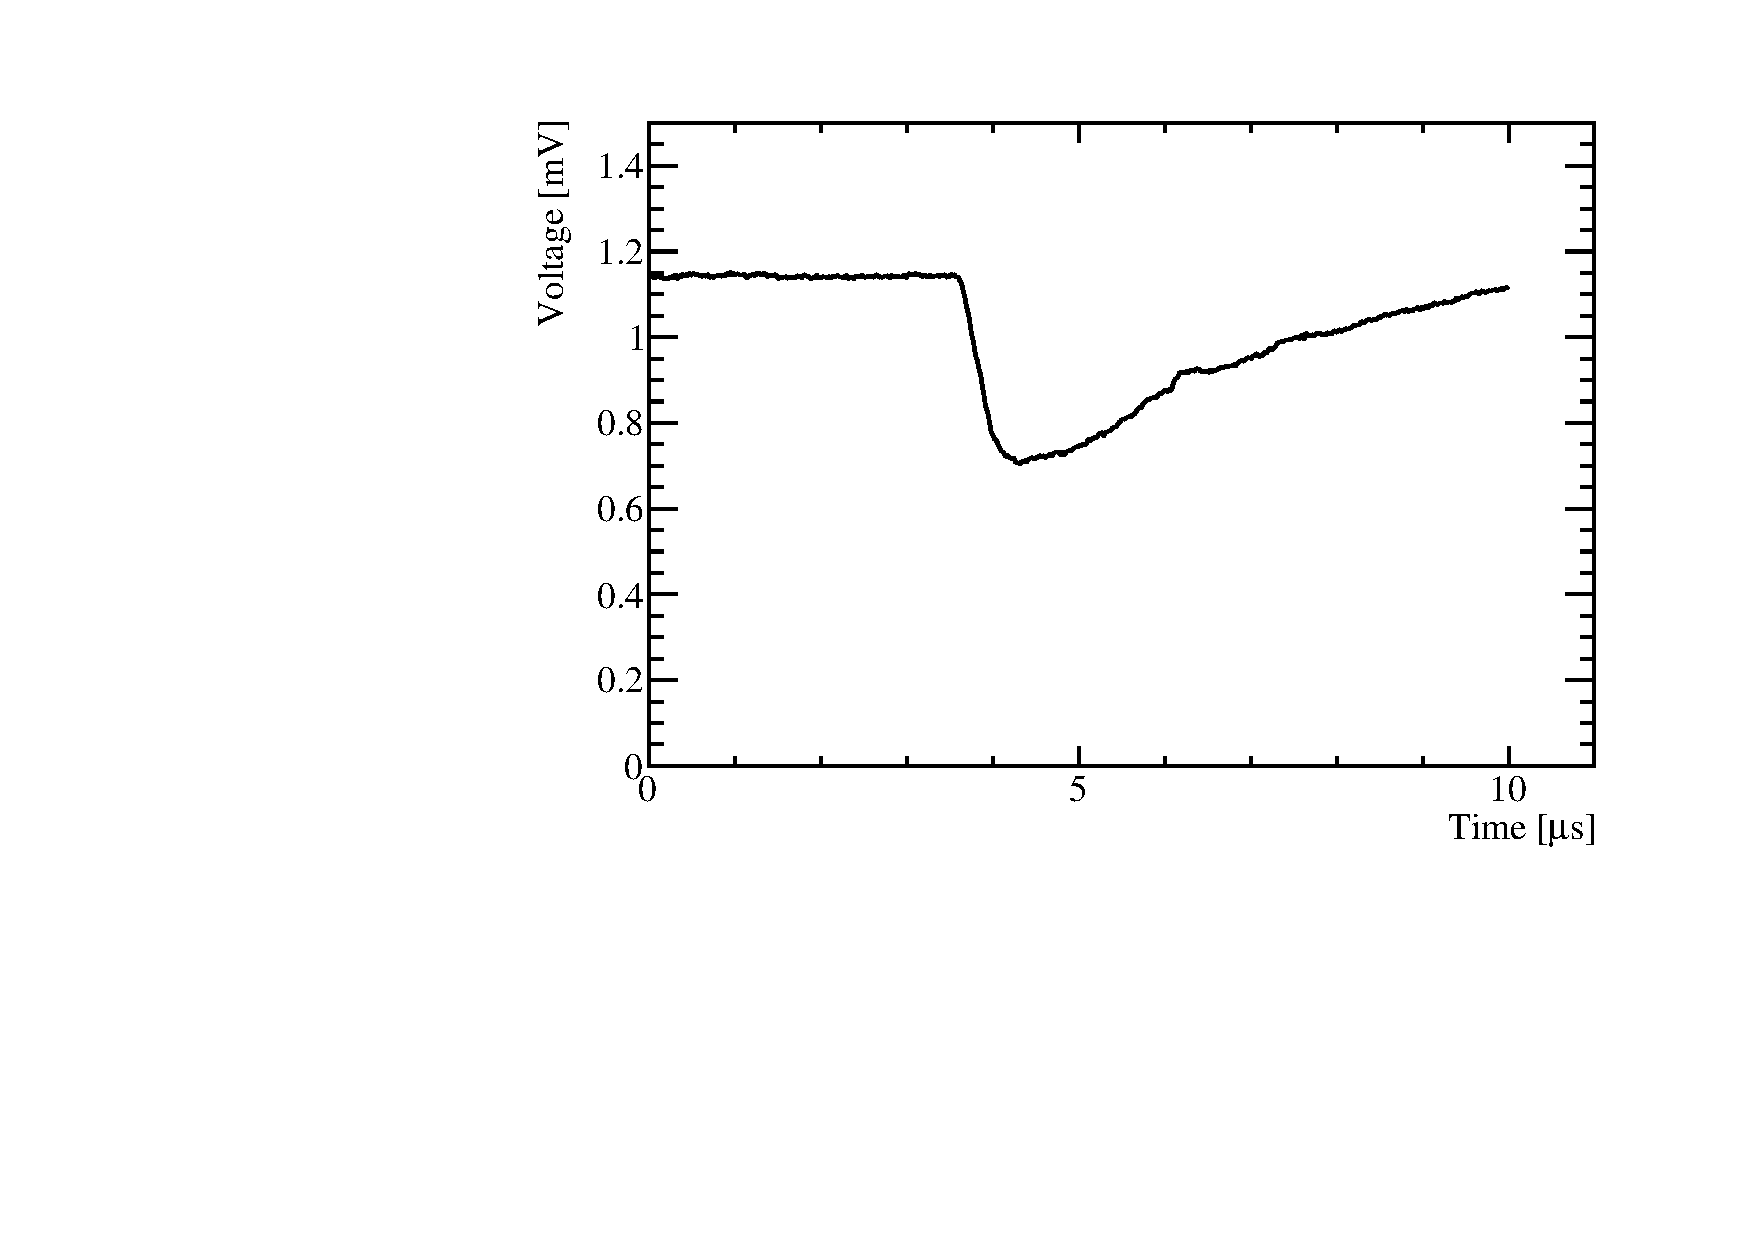
\includegraphics[width=0.5\textwidth]{CLICdpVertex/Plots/HV-CMOS/Frames/PulseShape01008NoOffset.pdf}}
\caption[HV-CMOS voltage as a function of time for pulses created by radioactive strontium 90 source.]{HV-CMOS voltage as a function of time for pulses created by radioactive $\text{Sr}^{90}$ source.}
\label{fig:pulseshapes}
\end{figure}

The HV-CMOS was biased to 60V during this experiment.  The HV-CMOS analogue output has a DC output of $\approx 1.15$ V and saturation occurs around a signal height of 700 mV.  Examples of the HV-CMOS output can be found in figure \ref{fig:pulseshapes}.

%========================================================================================

\subsubsection{Analysis}
The quantities of interest related to the HV-CMOS output are the pulse height and a rise time.  The offset voltage was subtracted from the HV-CMOS analogue output and the pulse height inverted before the following analysis was applied.

\begin{figure}
\centering
\subfloat[\textbf{Rise time.}  The blue arrows show the change in time and voltage as the pulse goes from 10\% to 90\% of the raw pulse height.  This time is used as the definition of the rise time in the subsequent analysis.]{\label{fig:pulseshapeanalysistime}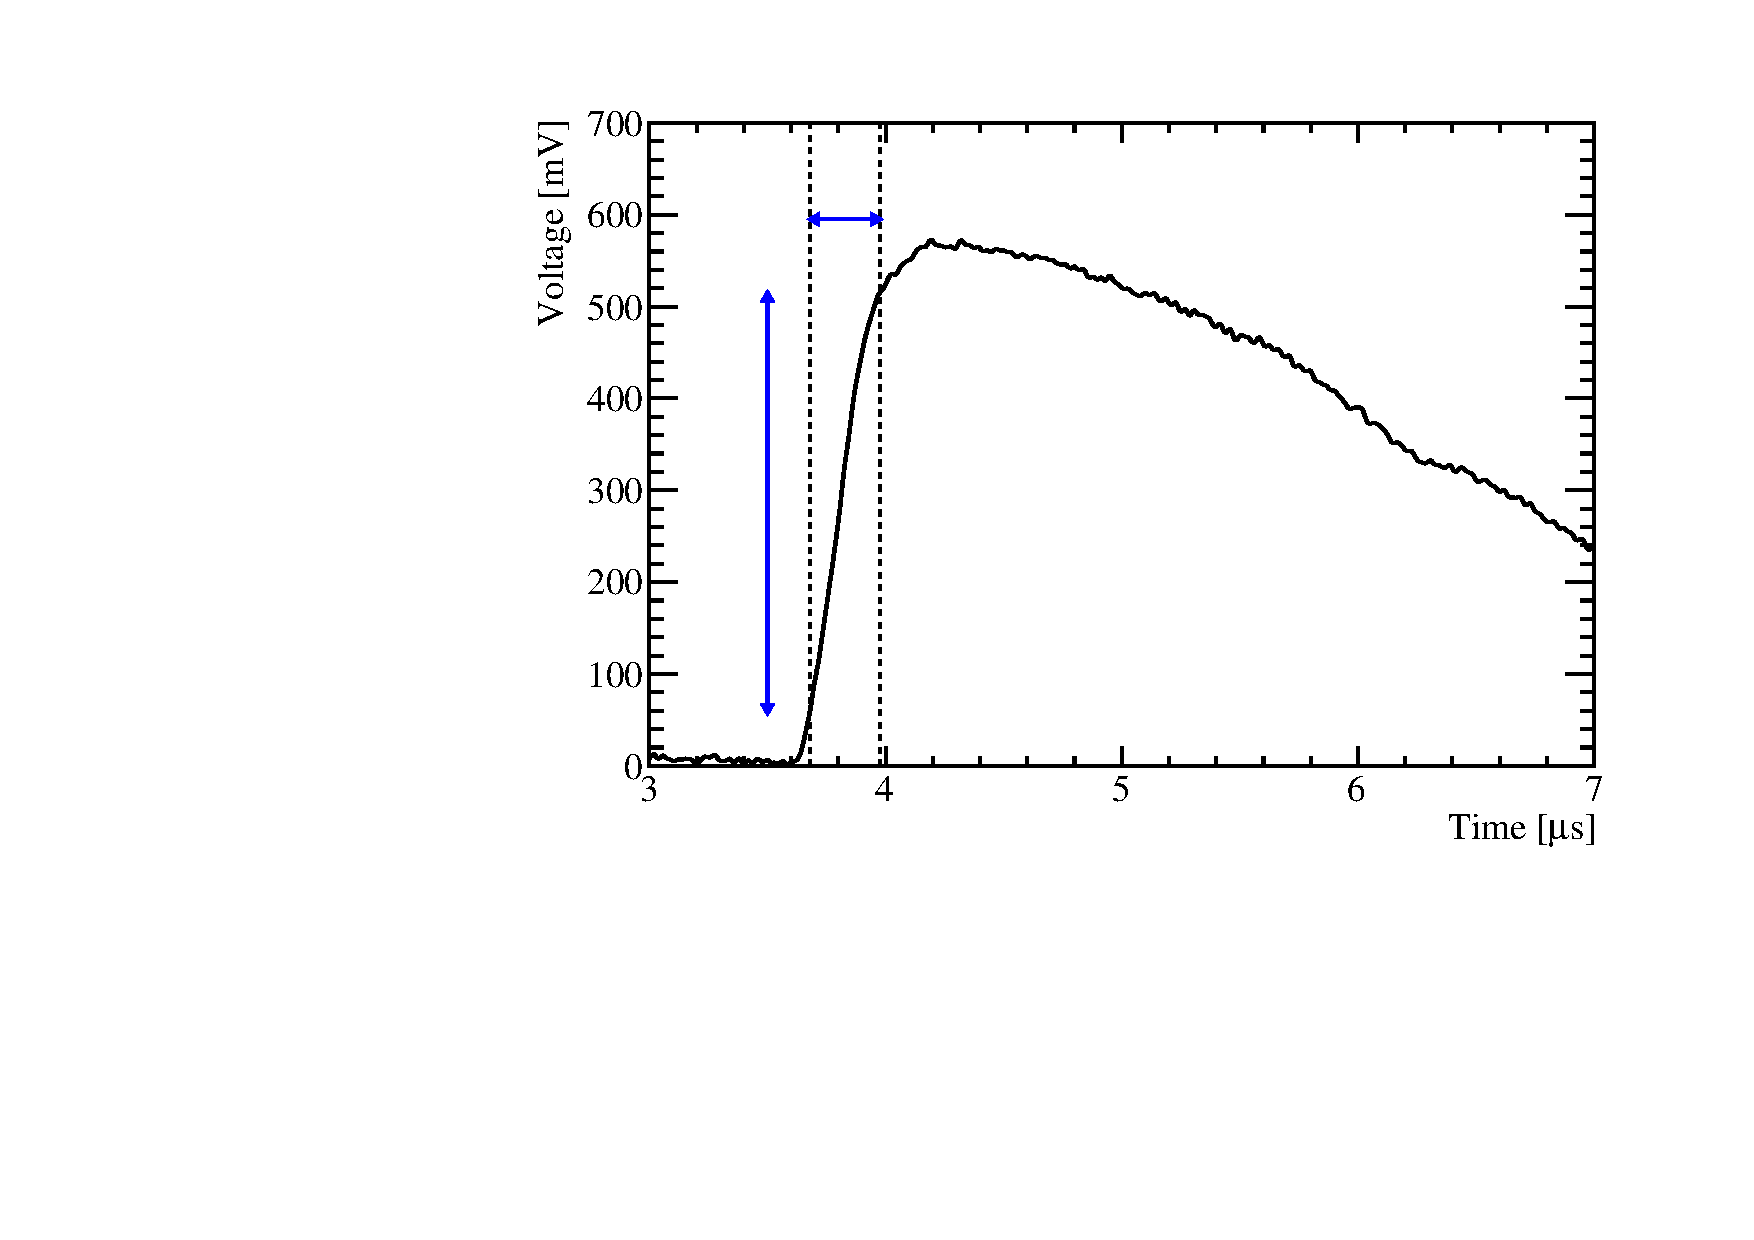
\includegraphics[width=0.5\textwidth]{CLICdpVertex/Plots/HV-CMOS/Frames/PulseShape01000FittingRiseTime.pdf}}
\subfloat[\textbf{Pulse height.} The red dotted line is a Gaussian fit to the peak of the pulse.  The peak is defined as data points where the voltage is in excess of 90\% of the raw pulse height.]{\label{fig:pulseshapeanalysisvoltage}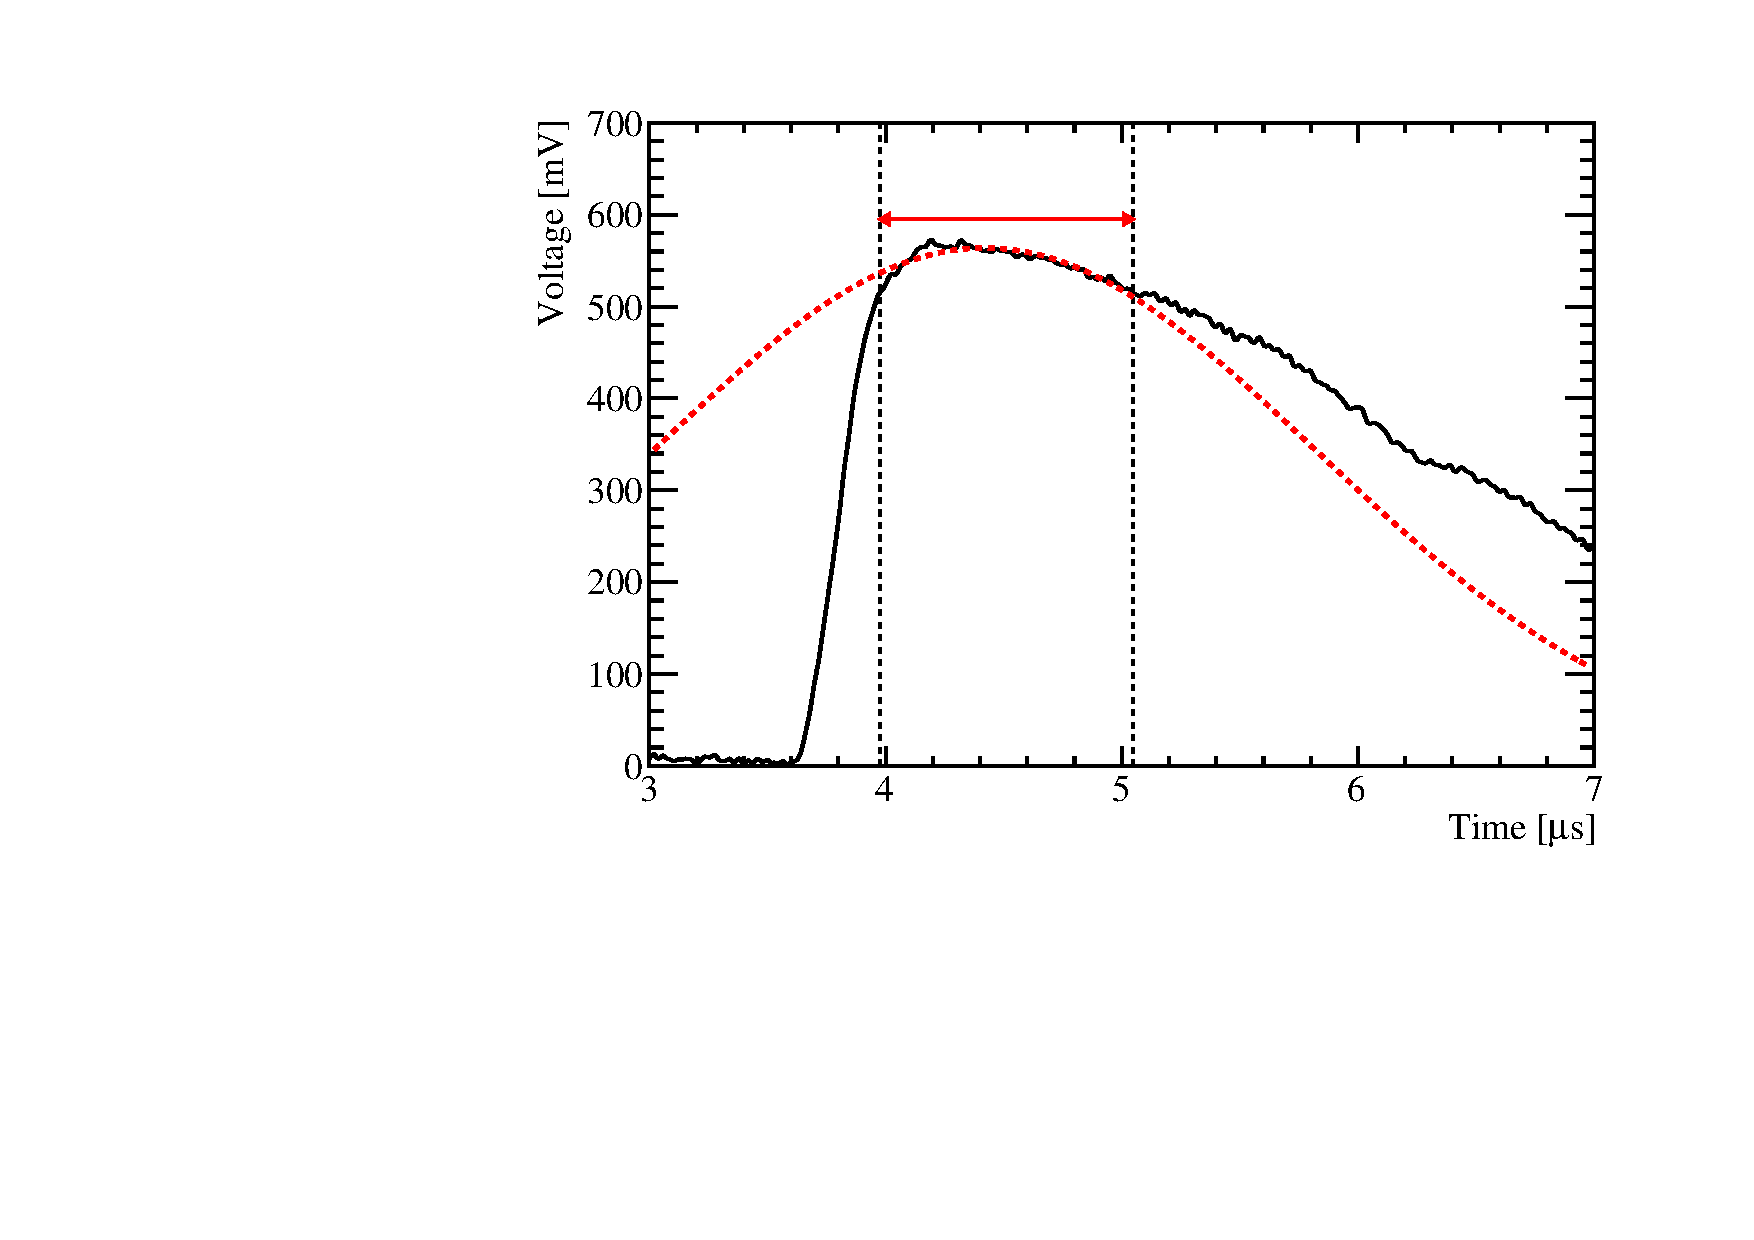
\includegraphics[width=0.5\textwidth]{CLICdpVertex/Plots/HV-CMOS/Frames/PulseShape01000FittingVoltage.pdf}}\hfill
\caption[Analysis of HV-CMOS voltage as a function of time for pulses created by radioactive strontium 90 source.]{Analysis of HV-CMOS voltage as a function of time for pulses created by radioactive $\text{Sr}^{90}$ source.}
\label{fig:pulseshapeanalysis}
\end{figure}

The pulse height was taken as the mean of a Gaussian fit to the peak of the HV-CMOS output voltage distribution.  The peak was defined as having a voltage change greater than 90\% of the maximum recorded voltage change.  The application of a Gaussian fit provides a more robust metric for categorising the pulse height, which is less dependant on fluctuations in the voltage.  The rise time was calculated as the time taken for the voltage to go from 10\% to 90\% of the maximum recorded voltage change.  This definition makes the rise time metric more robust against fluctuations in the voltage.  Examples of the calculation of these metrics for a given pulse are shown in figure \ref{fig:pulseshapeanalysis}.

For each device the HV-CMOS pulse output was recorded for 15 pixels running along one edge of the 64 $\times$ 64 matrix and in the subsequent analysis the data for all 15 pixels was combined.

%========================================================================================

\subsubsection{Results -  Rise Time vs Pulse Height}
\label{sec:resultsrisetimepulseheight}
The mean rise time as function of pulse height is shown in figure \ref{fig:risetime}.  This was determined by binning the events in terms of pulse height and determining the mean rise time for events in each of those bins.  The pulse height was binned using a bin width of 4 mV ranging from 0 to 700 mV.  At least 100 measurements per pulse height bin were used for the calculation of the average rise time.  The error bars on this figure show the standard error in the mean rise time.  

\begin{figure}
\centering
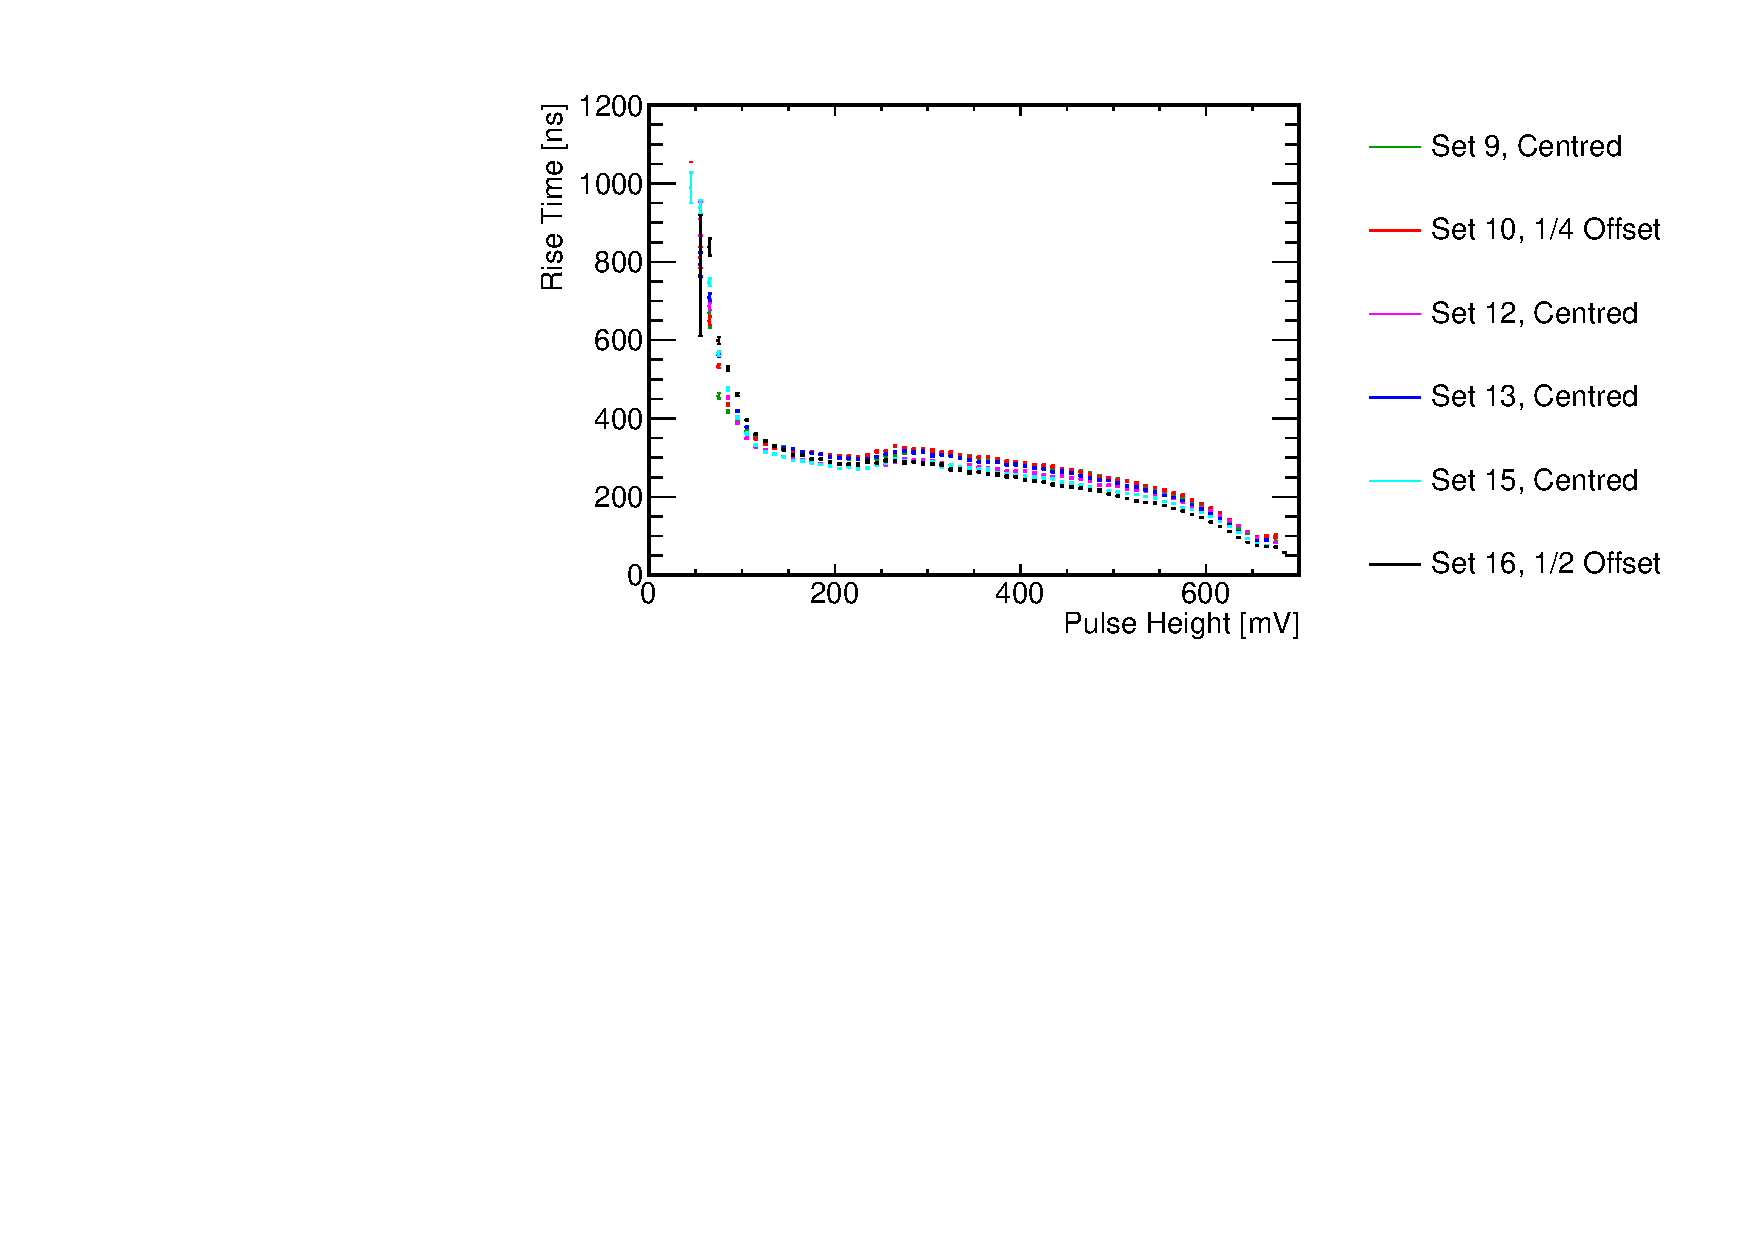
\includegraphics[width=1.0\textwidth]{CLICdpVertex/Plots/RadSourceAnalysis/AllSETs_RiseTime_PulseHeight.pdf}
\caption[HV-CMOS voltage rise time as a function of pulse height.]{HV-CMOS voltage rise time as a function of pulse height.}
\label{fig:risetime}
\end{figure}

The data in figure \ref{fig:risetime} indicates that the rise time is approximately 300 ns across all samples considered and that this is largely independent of pulse height for all but the largest and smallest values.  As the pulse height increase the rise time decreases, which is to be expected as the pulse heights are proportional to the signal from the $\text{e}^{-}$ and the larger this signal the larger the rate of change of output voltage from the HV-CMOS and so the lower the rise time.  For very small pulse heights, $< 100$ mV, the rise times are significantly larger indicating that the collected signal charge is taking a long time to be collected.  This is likely to be due to the signal charge travelling via diffusion rather than drift, which increases the time for the signal charge to be collected.  It is encouraging that all HV-CMOS devices have similar characteristics as it makes comparison of samples having different offsets between the HV-CMOS and the CLICpix ASIC possible.  This assumes the CLICpix sensors also behave in a similar manor across all samples considered, which is the case as the results in section \ref{testpulsecalibrationresults} show.  

%========================================================================================

\subsubsection{Results -  ToT vs Pulse Height}
\label{sec:totvspulseheight}
Figure \ref{fig:tot} shows the mean ToT as a function of pulse height.  The determination of the mean and error bars for the ToT measurement is identical to that described in section \ref{sec:resultsrisetimepulseheight} for the rise time measurement. 

\begin{figure}
\centering
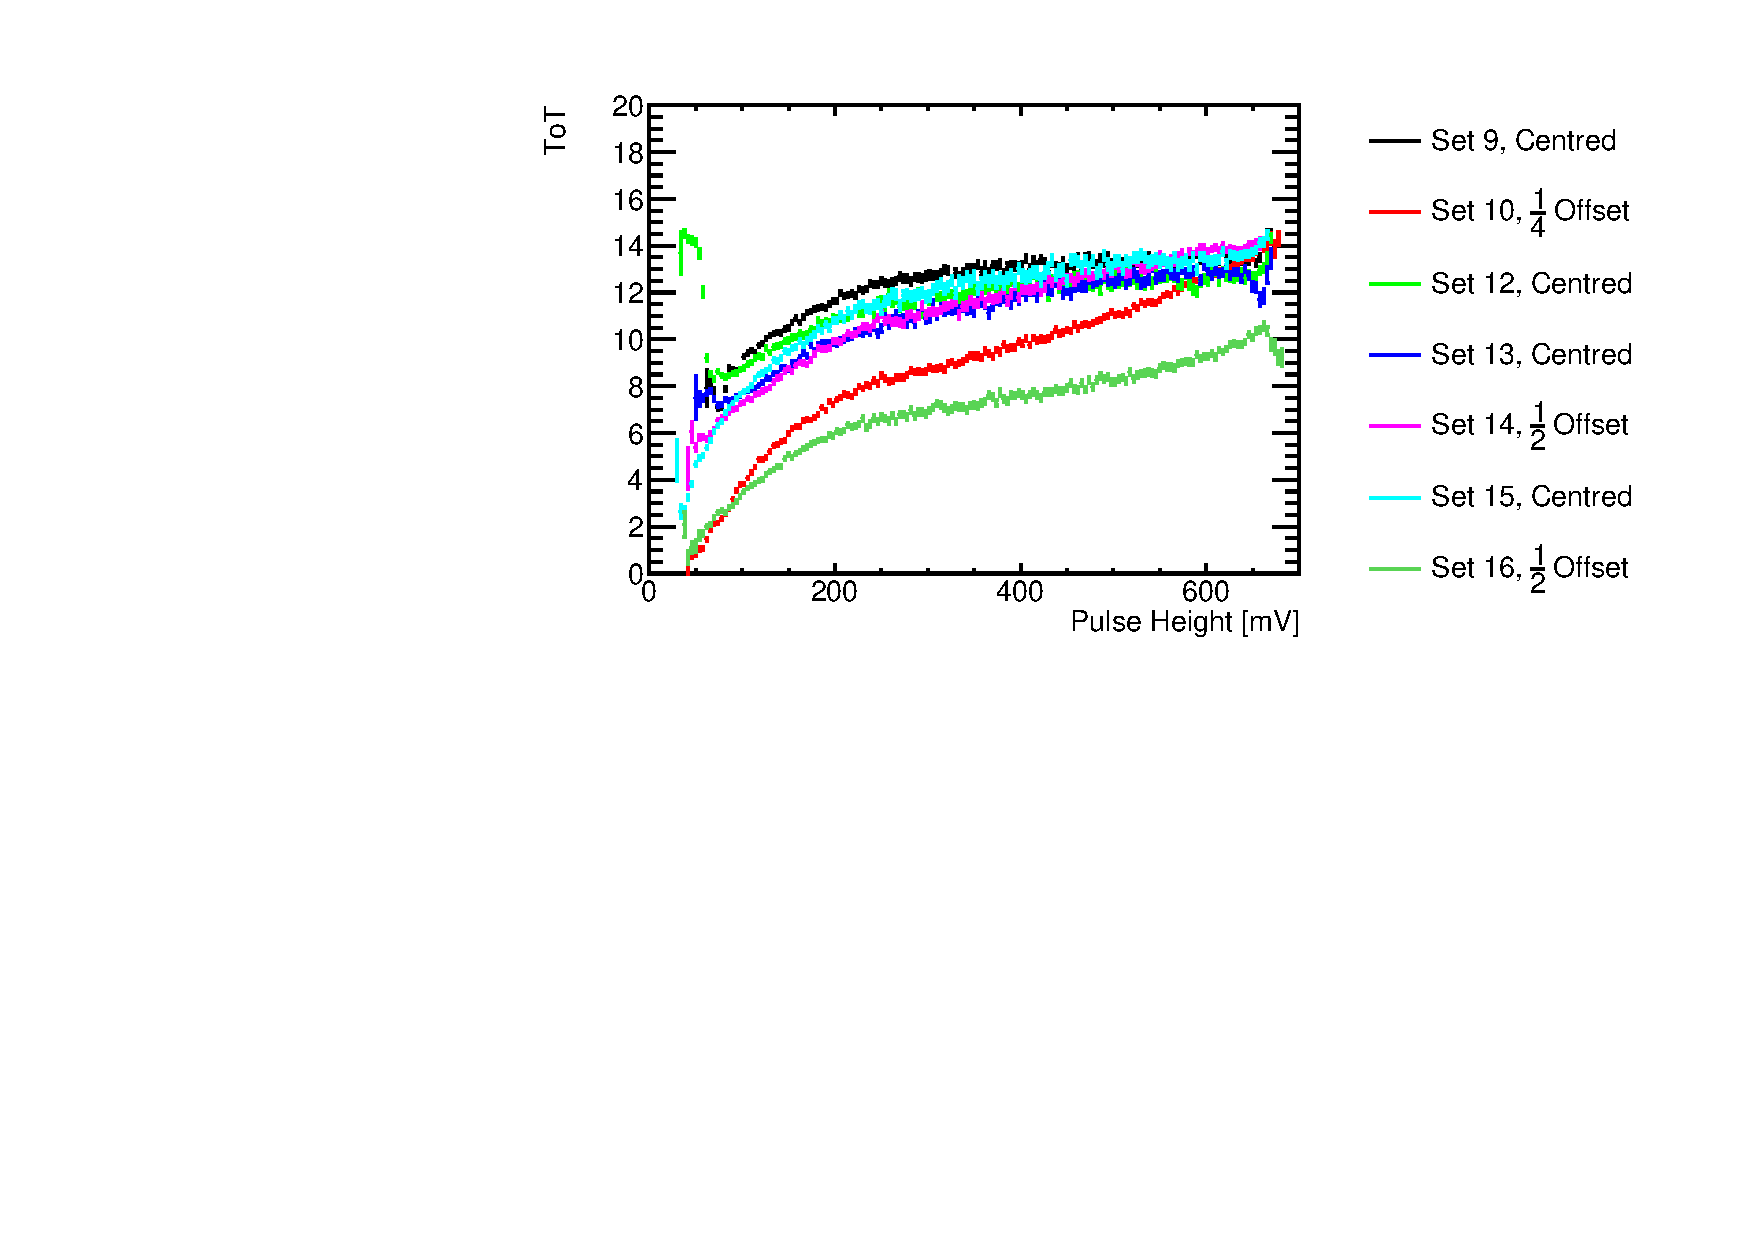
\includegraphics[width=1.0\textwidth]{CLICdpVertex/Plots/RadSourceAnalysis/AllSETs_TargetTot_PulseHeight.pdf}
\caption[CLICpix ToT as a function of HV-CMOS voltage pulse height.]{CLICpix ToT as a function of HV-CMOS voltage pulse height.}
\label{fig:tot}
\end{figure}

The distribution of mean ToT against pulse height shows that for centred samples the ToT increases with pulse height up to pulse heights of approximately 300 mV upon and that the mean ToT saturates at $\approx 13$ units.  It is expected that the $\frac{1}{4}$ and $\frac{1}{2}$ offset samples should have a lower ToT than the centred samples due to the lower effective capacitance between the HV-CMOS and the target CLICpix ASIC.  The greater the offset the smaller the effective capacitance to the target CLICpix and so the lower the recorded ToT.  This is what is observed when comparing the centred samples to the $\frac{1}{4}$ offset sample and one, Set 16, of the $\frac{1}{2}$ offset samples.  The other $\frac{1}{2}$ offset sample, Set 14, appears to behave as a centred sample indicating that this sample may have been manufactured with no offset.  

%========================================================================================

\subsubsection{Results -  Cross Couplings}
It is possible to further understand the splitting of the HV-CMOS signal between multiple CLICpix ASICs by examining the ToT on adjacent pixels, along the direction of the offset, as a function of the HV-CMOS pulse height.  This is shown in figure \ref{fig:totcrosscoupling1} for all devices that are centred and Set 14, which behaves as a centred device, and in figure \ref{fig:totcrosscoupling2} for the $\frac{1}{4}$ offset sample and the remaining $\frac{1}{2}$ offset sample, Set 16.  

No correlation between the adjacent pixel ToT and the HV-CMOS pulse height is observed for the samples shown in figure \ref{fig:totcrosscoupling1} for all but the lowest values of pulse height.  The correlation observed at low pulse heights may arise due to the signal $\text{e}^{-}$, which is primarily recorded in the target pixel, depositing a small amount of charge in the adjacent adjacent pixel.  This can happen as the $\text{e}^{-}$ may not be traveling normal to the pixel surface.  However, as this feature is not present in all samples it could indicate a small misalignment exists in the samples showing the correlation.  

There is, however, a strong correlation between adjacent pixel ToT and the HV-CMOS pulse height, shown in figure \ref{fig:totcrosscoupling2}, for Set 16, which is one of the $\frac{1}{2}$ offset samples.  This distribution is almost identical to the the target pixel ToT distribution as a function of HV-CMOS pulse height, which is what would be expected given an equal signal charge sharing between the two readout ASICs.  This indicates the charge sharing is well understood for this $\frac{1}{2}$ offset sample.   

For the $\frac{1}{4}$ offset sample correlation is present only for low pulse heights as was the case for the centred samples.  However, the mean ToT within the uncorrelated region is centred around $\approx$ 5 units of ToT, which is lower than was observed for the centred samples.  This is due to the offset reducing the total capacitance between the HV-CMOS and CLICpix in comparison to the centred samples and thus reducing the ToT recorded.

Cross coupling was observed in one of the $\frac{1}{2}$ offset samples and, assuming that the other $\frac{1}{2}$ offset sample was manufactured incorrectly, then charge sharing was well understood for these $\frac{1}{2}$ offset samples.  No cross coupling was observed for any of the other samples considered in this analysis.  

\begin{figure}
\centering
\subfloat[]{\label{fig:totcrosscoupling1}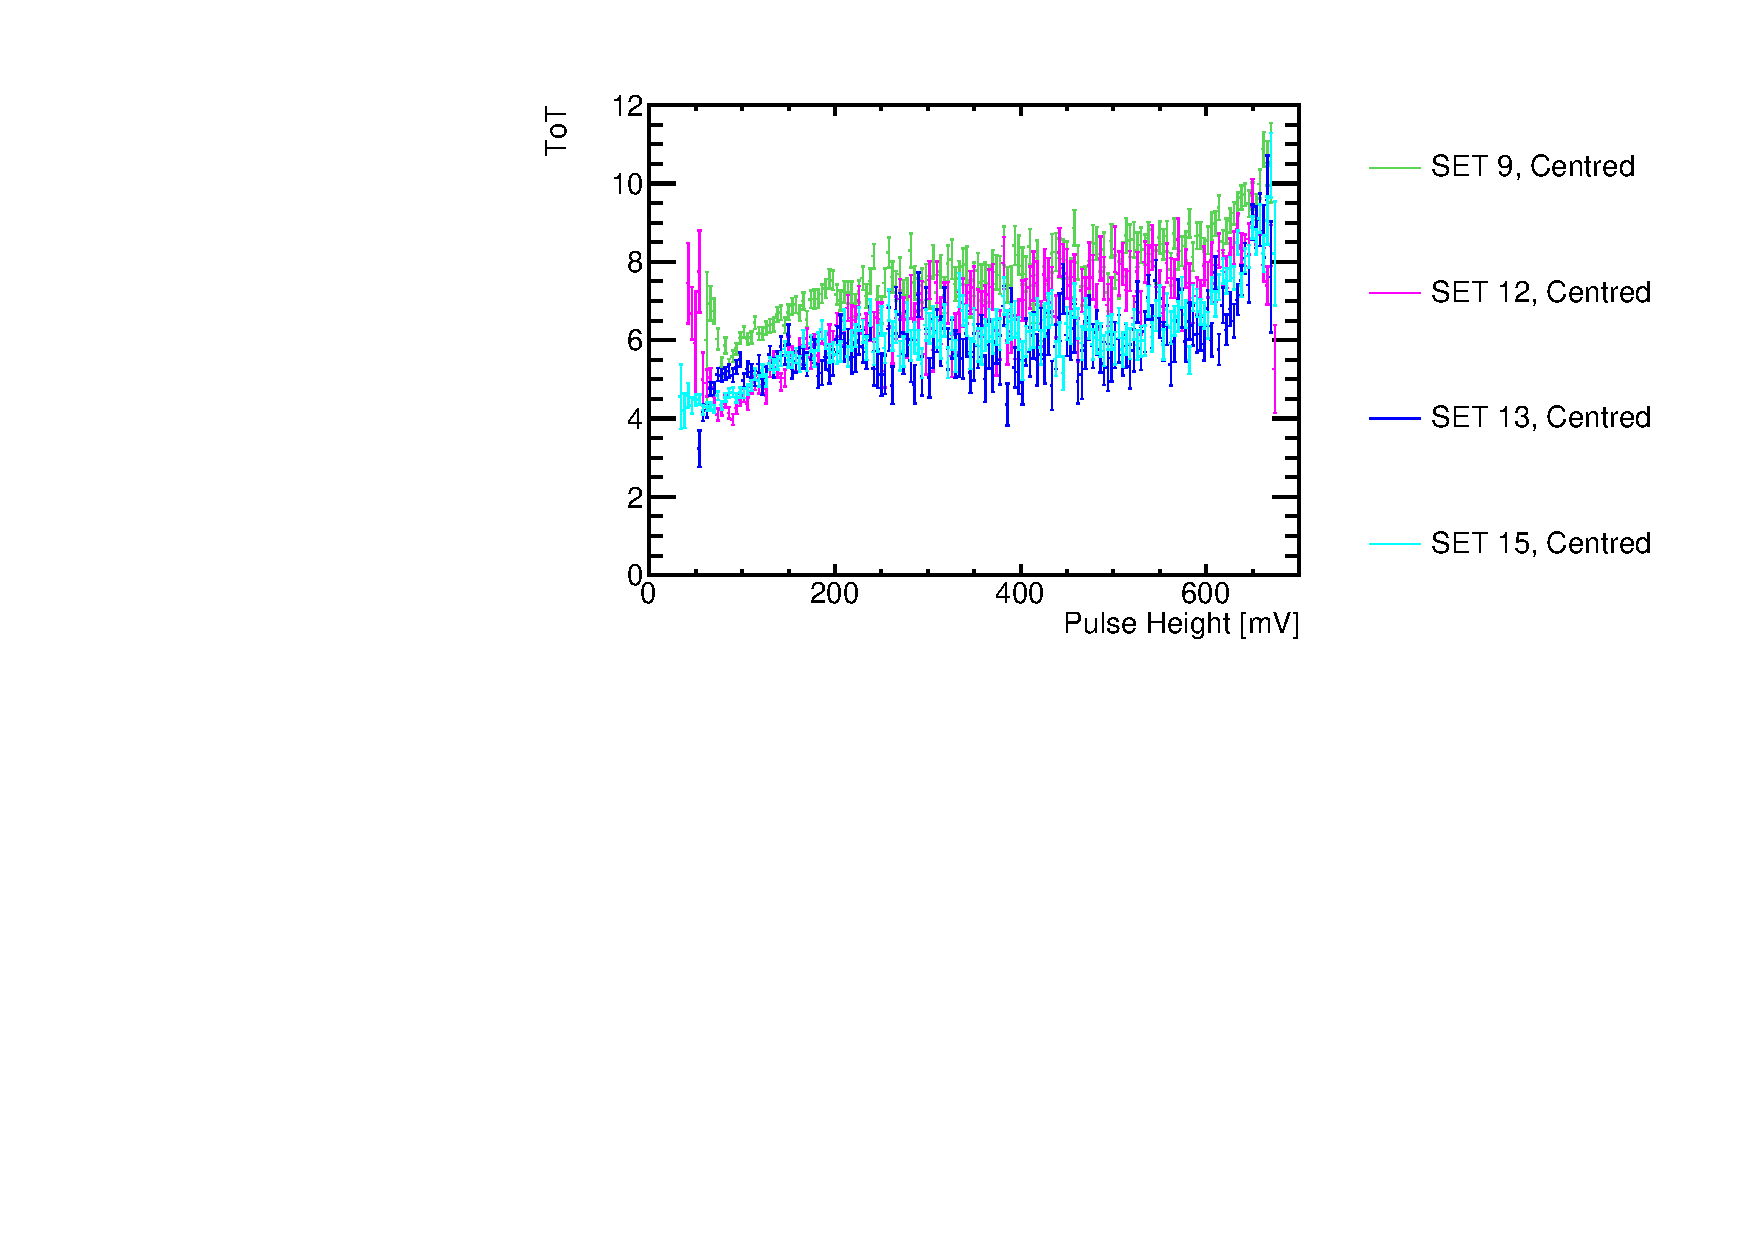
\includegraphics[width=1.0\textwidth]{CLICdpVertex/Plots/RadSourceAnalysis/NoCrossCouplingSETs_Tot_X_PulseHeight.pdf}}\hfill
\subfloat[]{\label{fig:totcrosscoupling2}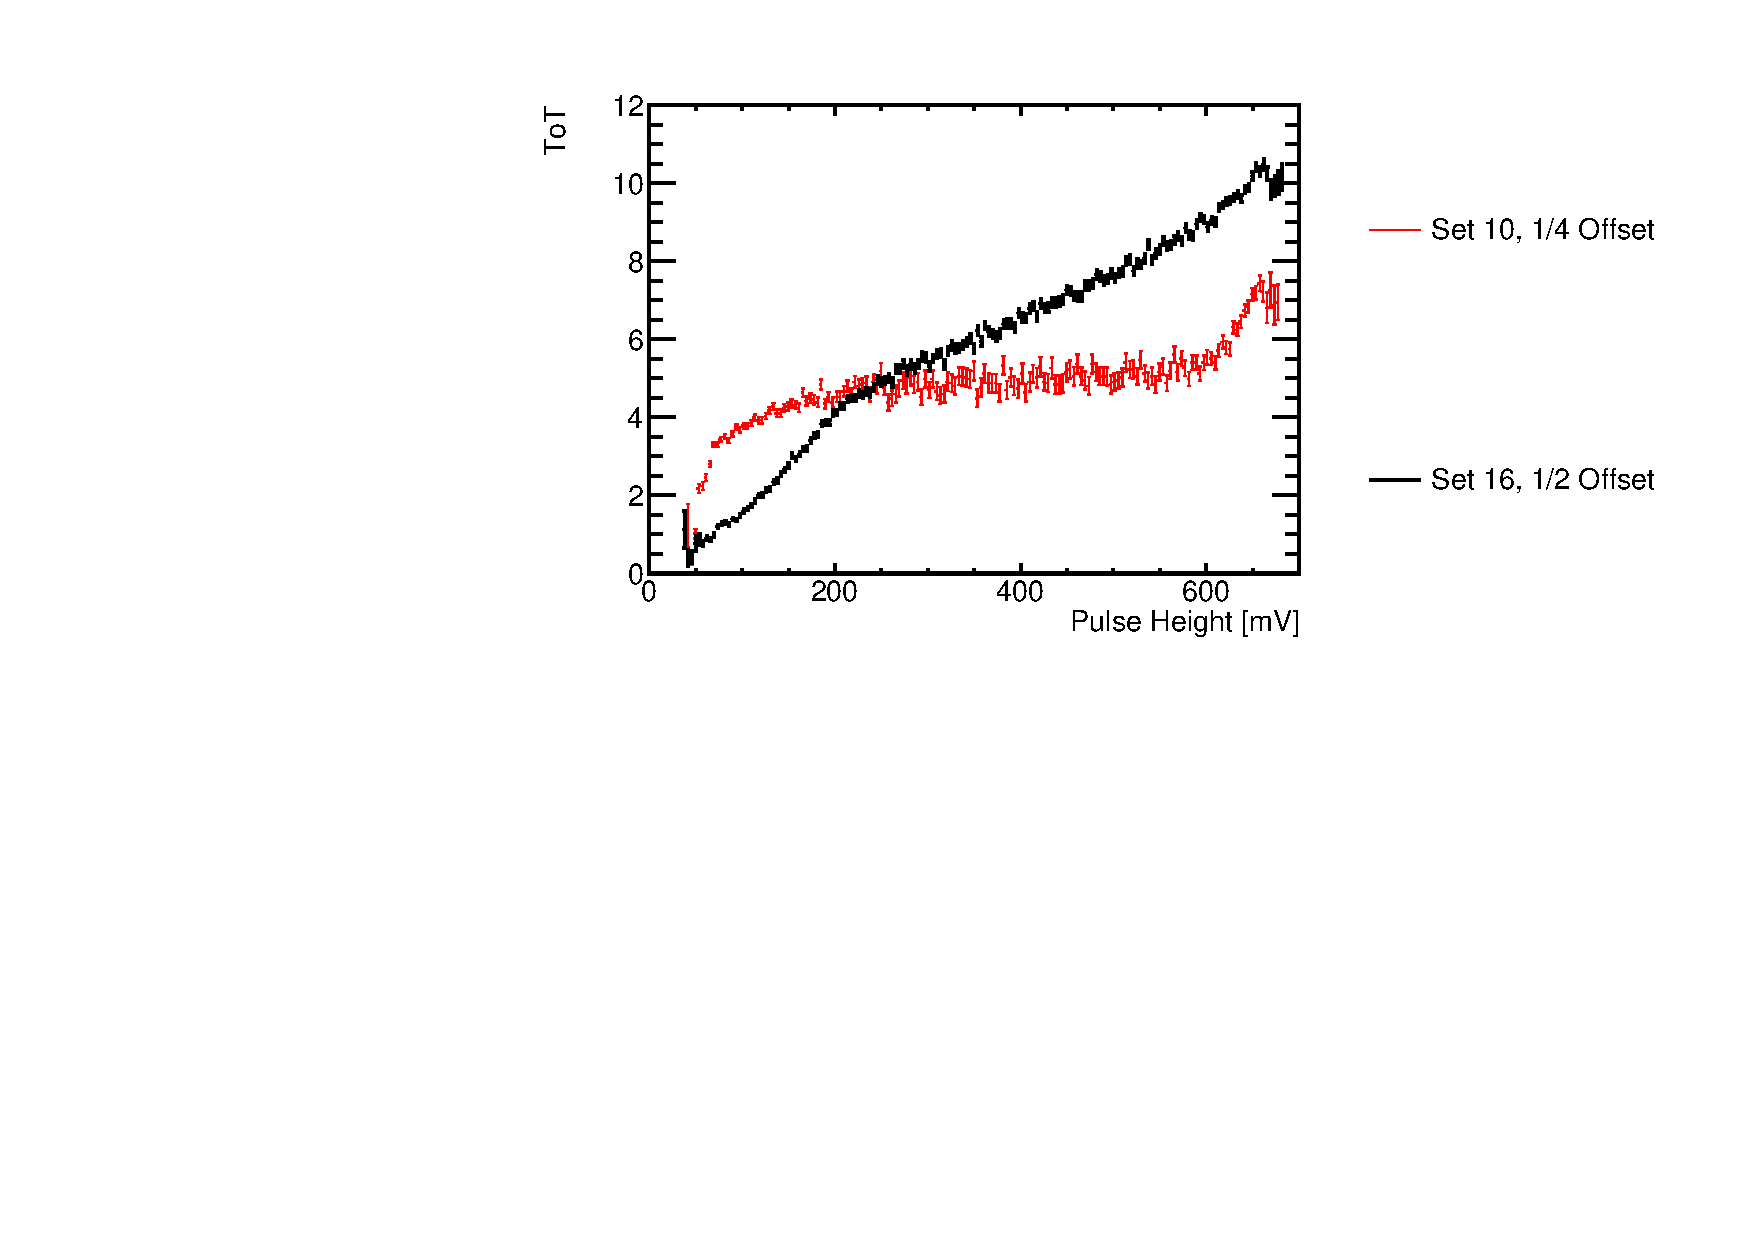
\includegraphics[width=1.0\textwidth]{CLICdpVertex/Plots/RadSourceAnalysis/CrossCouplingSETs_Tot_X_PulseHeight.pdf}}
\label{fig:totcrosscoupling}
\caption[CLICpix ToT on adjacent pixel along the direction of the offset as a function of HV-CMOS voltage pulse height.]{CLICpix ToT on adjacent pixel along the direction of the offset as a function of HV-CMOS voltage pulse height.}
\end{figure}

%========================================================================================

\subsection{Test Pulse Calibration}
The next test that was performed involved directly injecting a voltage pulse of fixed height directly into the CLICpix ASIC, which gives a measure of the performance of the CLICpix independently of the HV-CMOS sensor.  Due to the construction of the sensor it was not possible to access the HV-CMOS to perform a similar test to isolate its performance.  

%========================================================================================

\subsubsection{Experimental Setup}
In this study a voltage pulse of fixed height was injected into 1 out of every 16 pixels from the matrix, while masking the others, and the ToT from the CLICpix recorded.  This repeated 15 more times using different mask configurations until the entire matrix had been samples.  The masking of pixels was done as to not overload the matrix by running all pixels at ones.  This procedure was repeated 100 times so that average ToTs could be recorded.  The pulse height injected into the CLICpix varied from 2 to 180 mV in steps of 2 mV.  An example of the mean ToT plotted against the injected pulse height is shown in figure \ref{fig:testpulseexamplenofit}.  

\begin{figure}
\centering
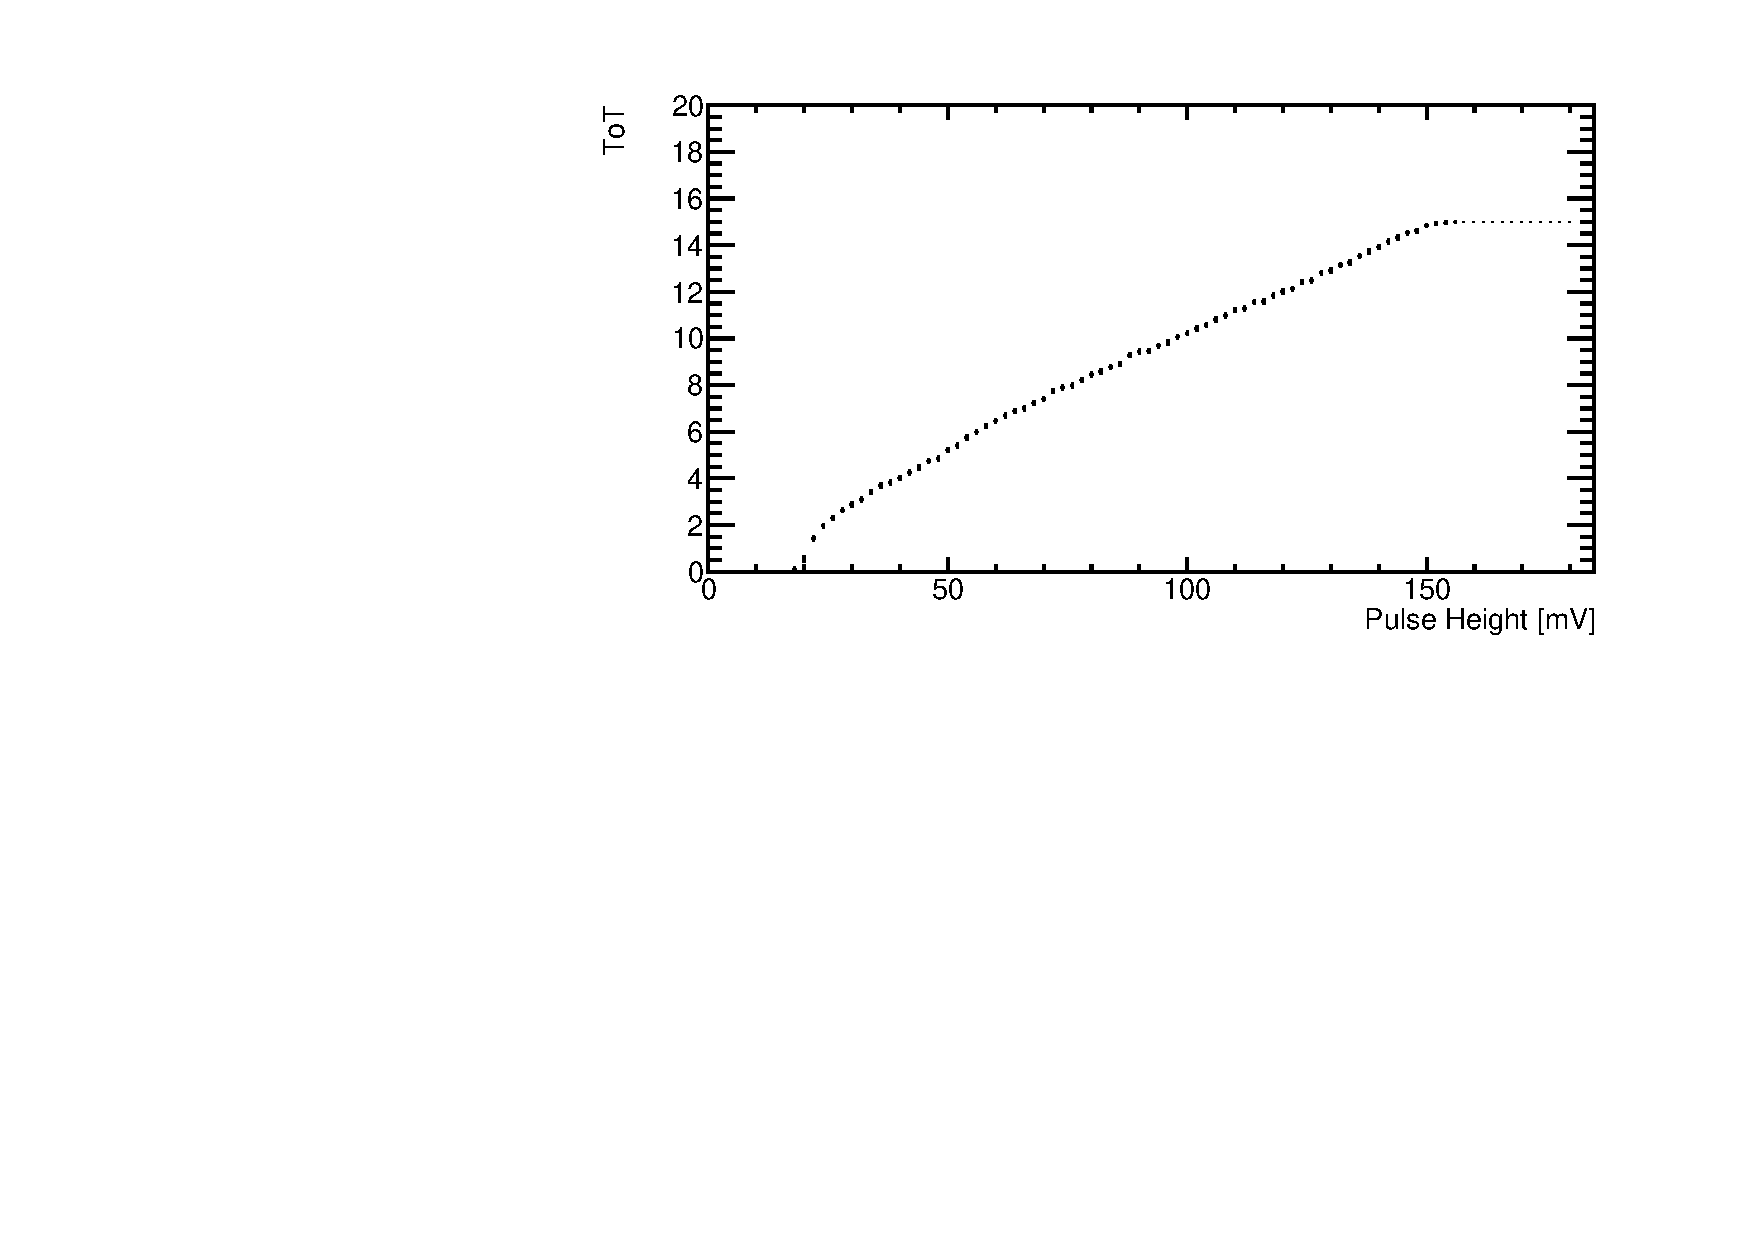
\includegraphics[width=1.0\textwidth]{CLICdpVertex/Plots/TestPulseCalibration/Fits/Set9/ToT_PulseHeight_Set_9_ChipID_001ec0db94b1_Pixel_x0_y0_NoFit.pdf}
\caption[CLICpix ToT as a function of injected pulse height.]{CLICpix ToT as a function of injected pulse height for a single pixel from a centred sample, Set 9.  The black markers are the mean ToT and the error bars are the standard error in the mean.  The solid red line shows the surrogate function fit and the dotted red lines show the range where the fit was applied.}
\label{fig:testpulseexamplenofit}
\end{figure}

%========================================================================================

\subsubsection{Analysis}
The functional form of the ToT against pulse height plot is described using the surrogate function \cite{AlipourTehrani:2054922}, which is defined as

\begin{equation}
y  = ax + b  - \frac{c}{x-t}
\end{equation}

where $y$ is the ToT, $x$ is the pulse height and $a$, $b$, $c$ and $d$ are fit parameters.  For large pulse heights the linear relationship dominated and for low pulse heights the inversely proportional term dominates.  $c$ describes the curvature of the graph, while $t$ determines the asymptote below which no signal is detected.  Figure \ref{fig:testpulseexamplefit} shows and example of the application of this fit.  As this function does not describe saturation of the ToT or the no signal region the fit is only applied on data points where the mean ToT is greater than 1 and less than 14.75.  

\begin{figure}
\centering
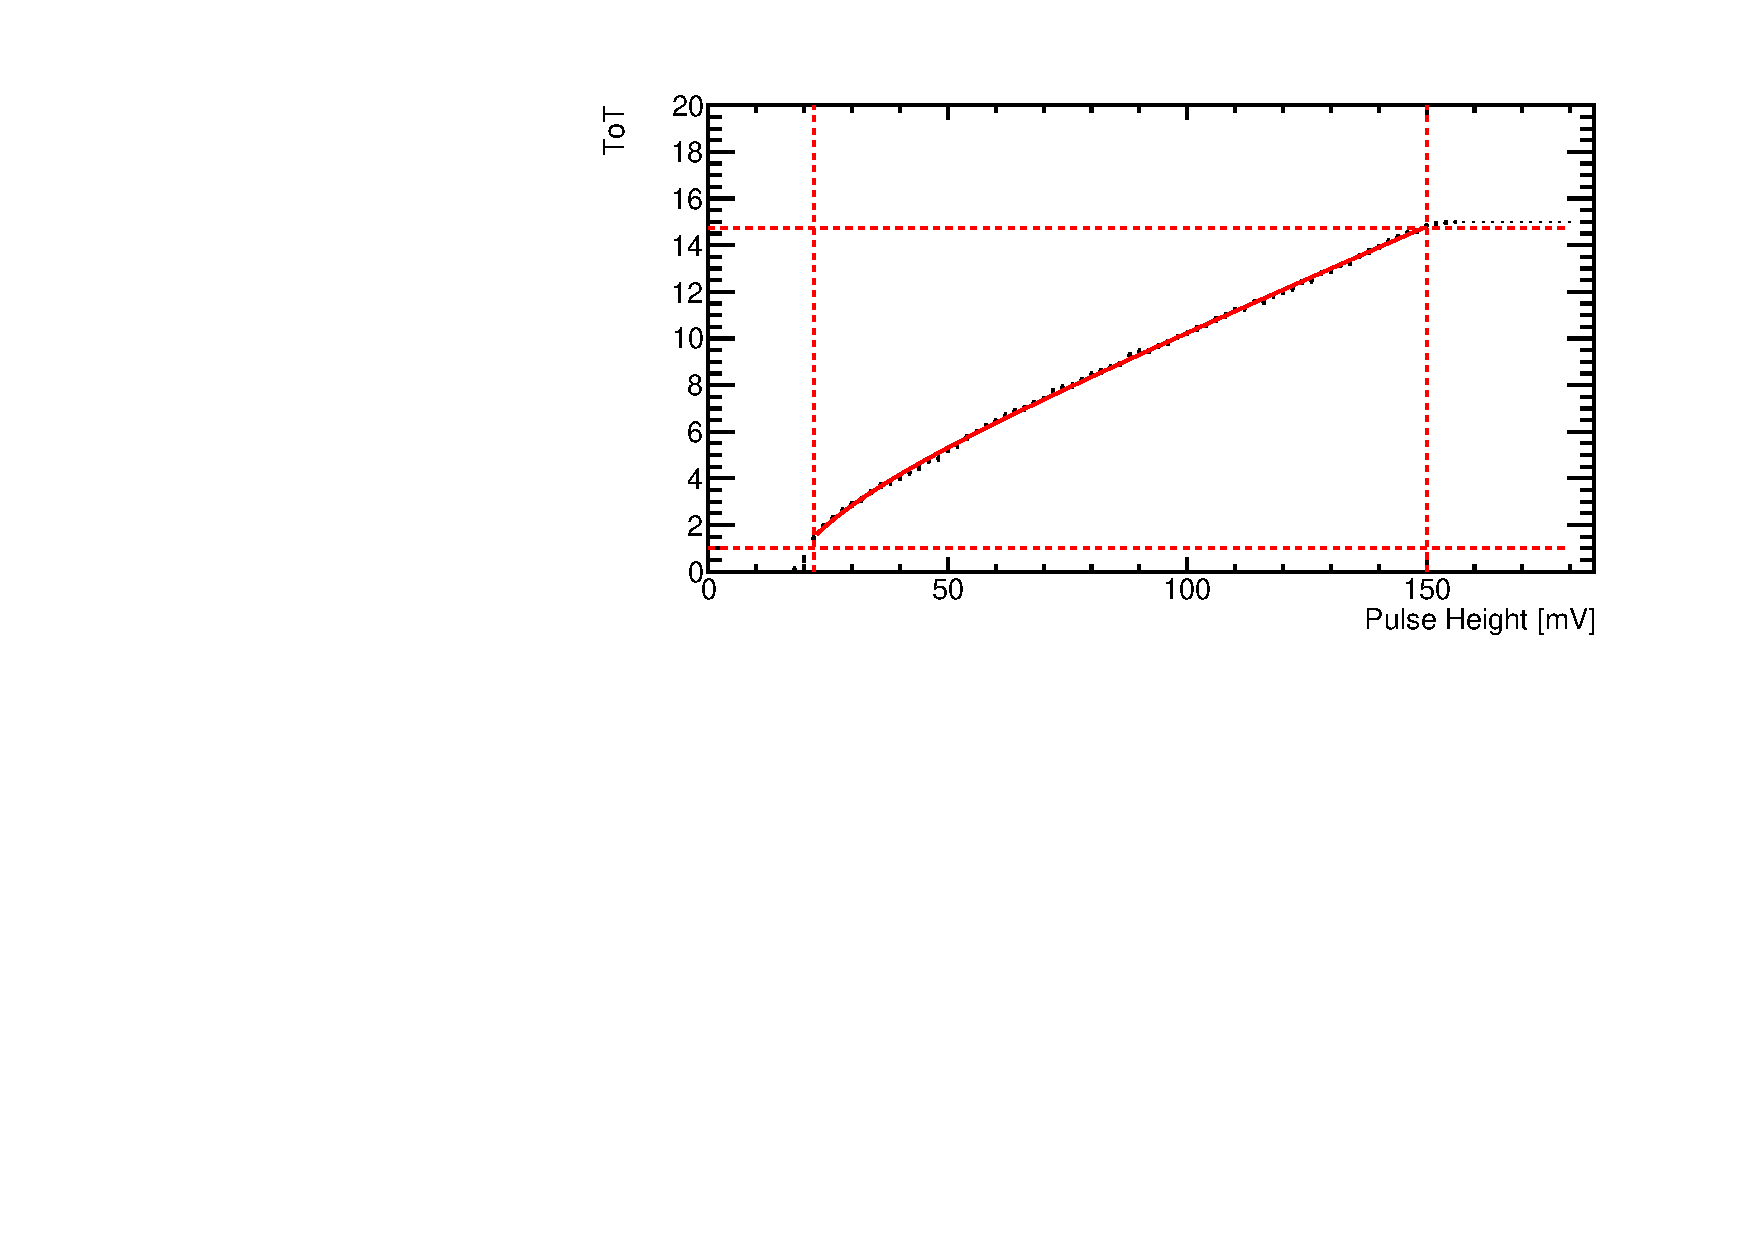
\includegraphics[width=1.0\textwidth]{CLICdpVertex/Plots/TestPulseCalibration/Fits/Set9/ToT_PulseHeight_Set_9_ChipID_001ec0db94b1_Pixel_x0_y0_Fit.pdf}
\caption[CLICpix ToT as a function of injected pulse height.]{CLICpix ToT as a function of injected pulse height for a single pixel from a centred sample, Set 9.  The black markers are the mean ToT and the error bars are the standard error in the mean.  The solid red line shows the surrogate function fit and the dotted red lines show the range where the fit was applied.}
\label{fig:testpulseexamplefit}
\end{figure}

The application of this fit condenses the information for individual pixels down to four parameters.  These parameters can be averaged to categorise the CLICpix response across the matrix.  

%========================================================================================

\subsubsection{Results}
\label{sec:testpulsecalibrationresults}
A known issue withe the design of the CLICpix ASIC is that there is a different bias on alternate columns of the matrix, which alters the shape of the ToT as a function of the injected pulse height.  In particular the different bias affects the minimum pulse height to get a response for the CLICpix, which is determined by parameters $c$ and $t$ in the surrogate function.  This feature can be observed by examining the distribution of the fit parameters.  These distributions are shown for sensor Set 9 in figure \ref{fig:fitparams}.  The peak at zero in the distribution of the $a$ and $b$ parameter, $\approx$ 150 in total, correspond to dead pixels in the sensor.  While the $a$ and $b$ parameters are centred around a single value indicating a similar response in the linear region of the surrogate function, the $c$ and $t$ parameters are centred around one of two values.  When examining the distribution of these parameters as a function of position on the matrix, shown in figure \ref{fig:fitparams2d} for Set 9, it can be seen that the structure is related to the column a given pixel is in.  This feature is present in all devices considered and will be removed for the next generation of the CLICpix ASIC.

\begin{figure}
\centering
\subfloat[$a$ parameter.]{\label{fig:fitparams1}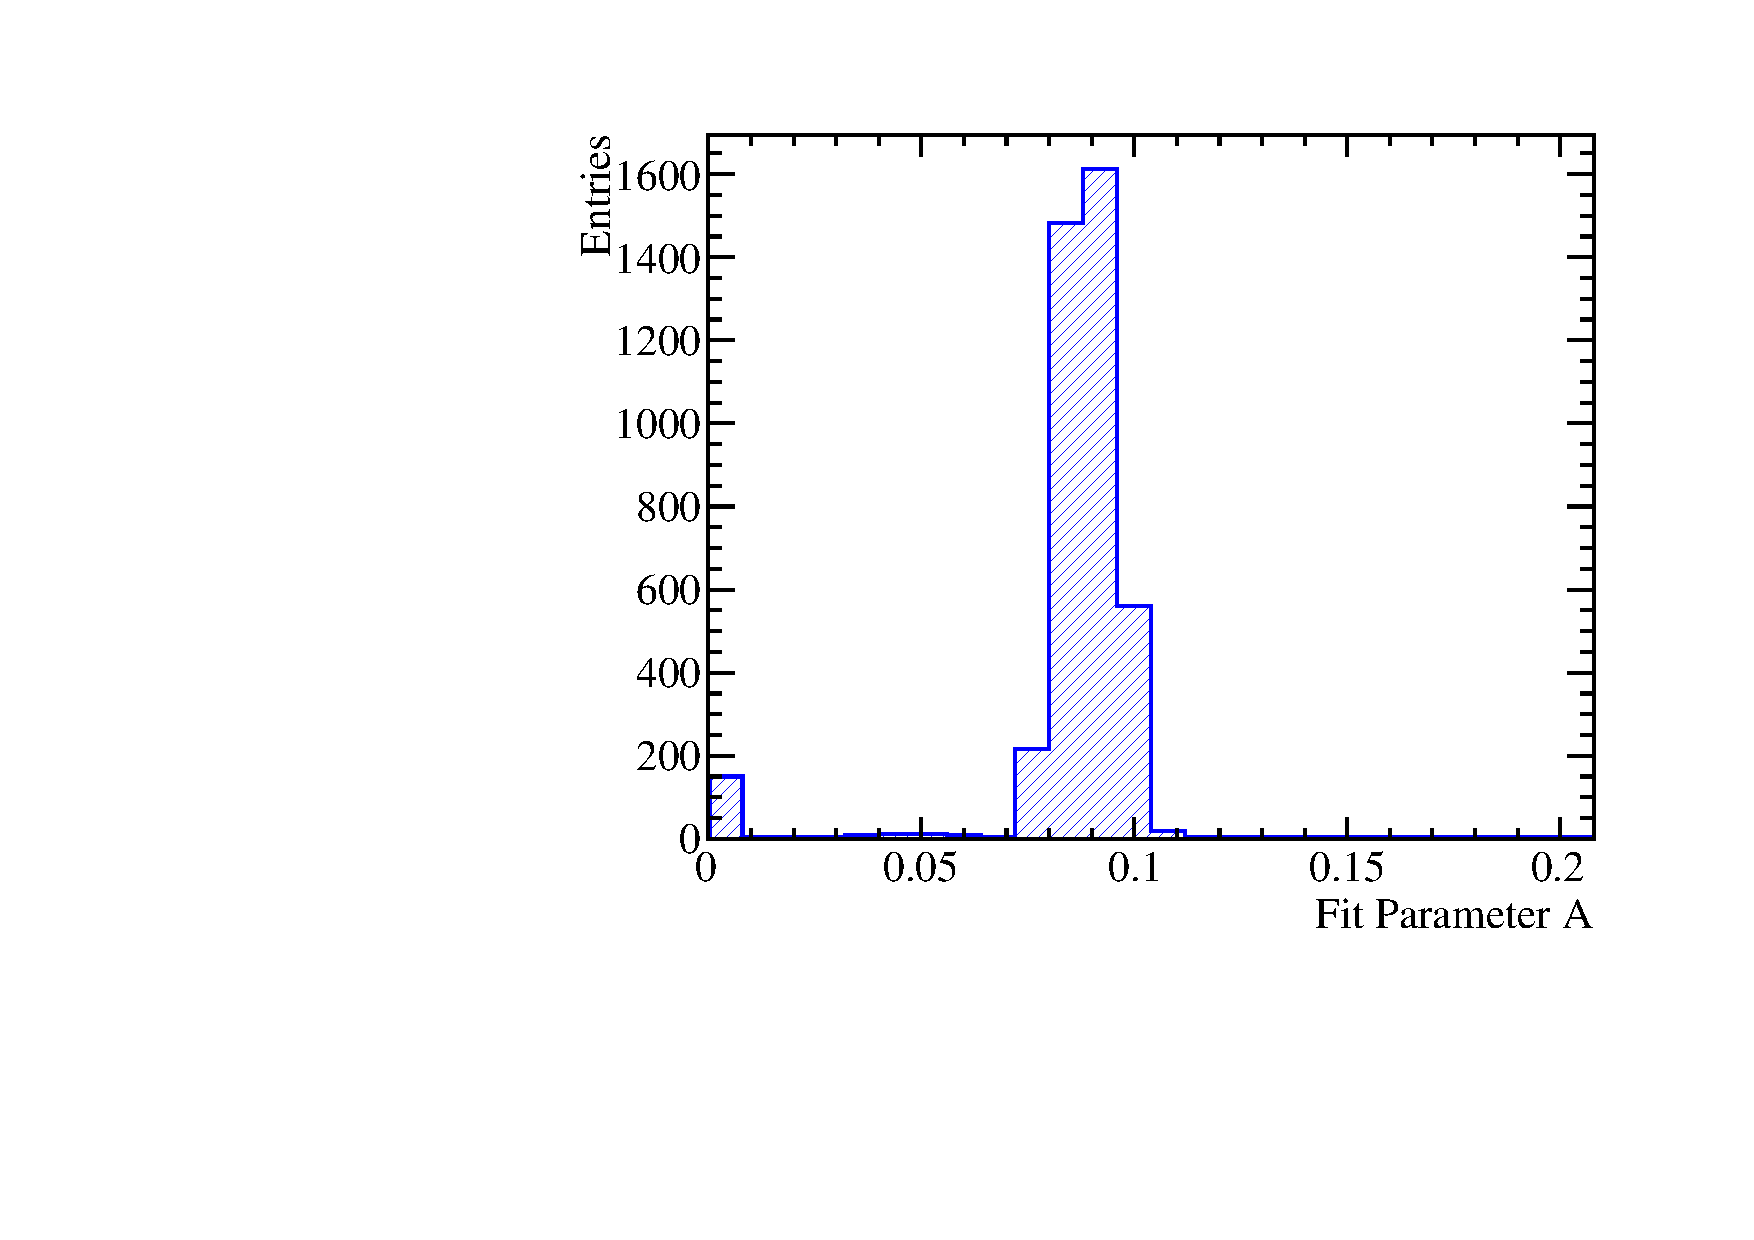
\includegraphics[width=0.5\textwidth]{CLICdpVertex/Plots/TestPulseCalibration/FitParam/OneDHistFitParamA_Set9.pdf}}
\subfloat[$b$ parameter.]{\label{fig:fitparams2}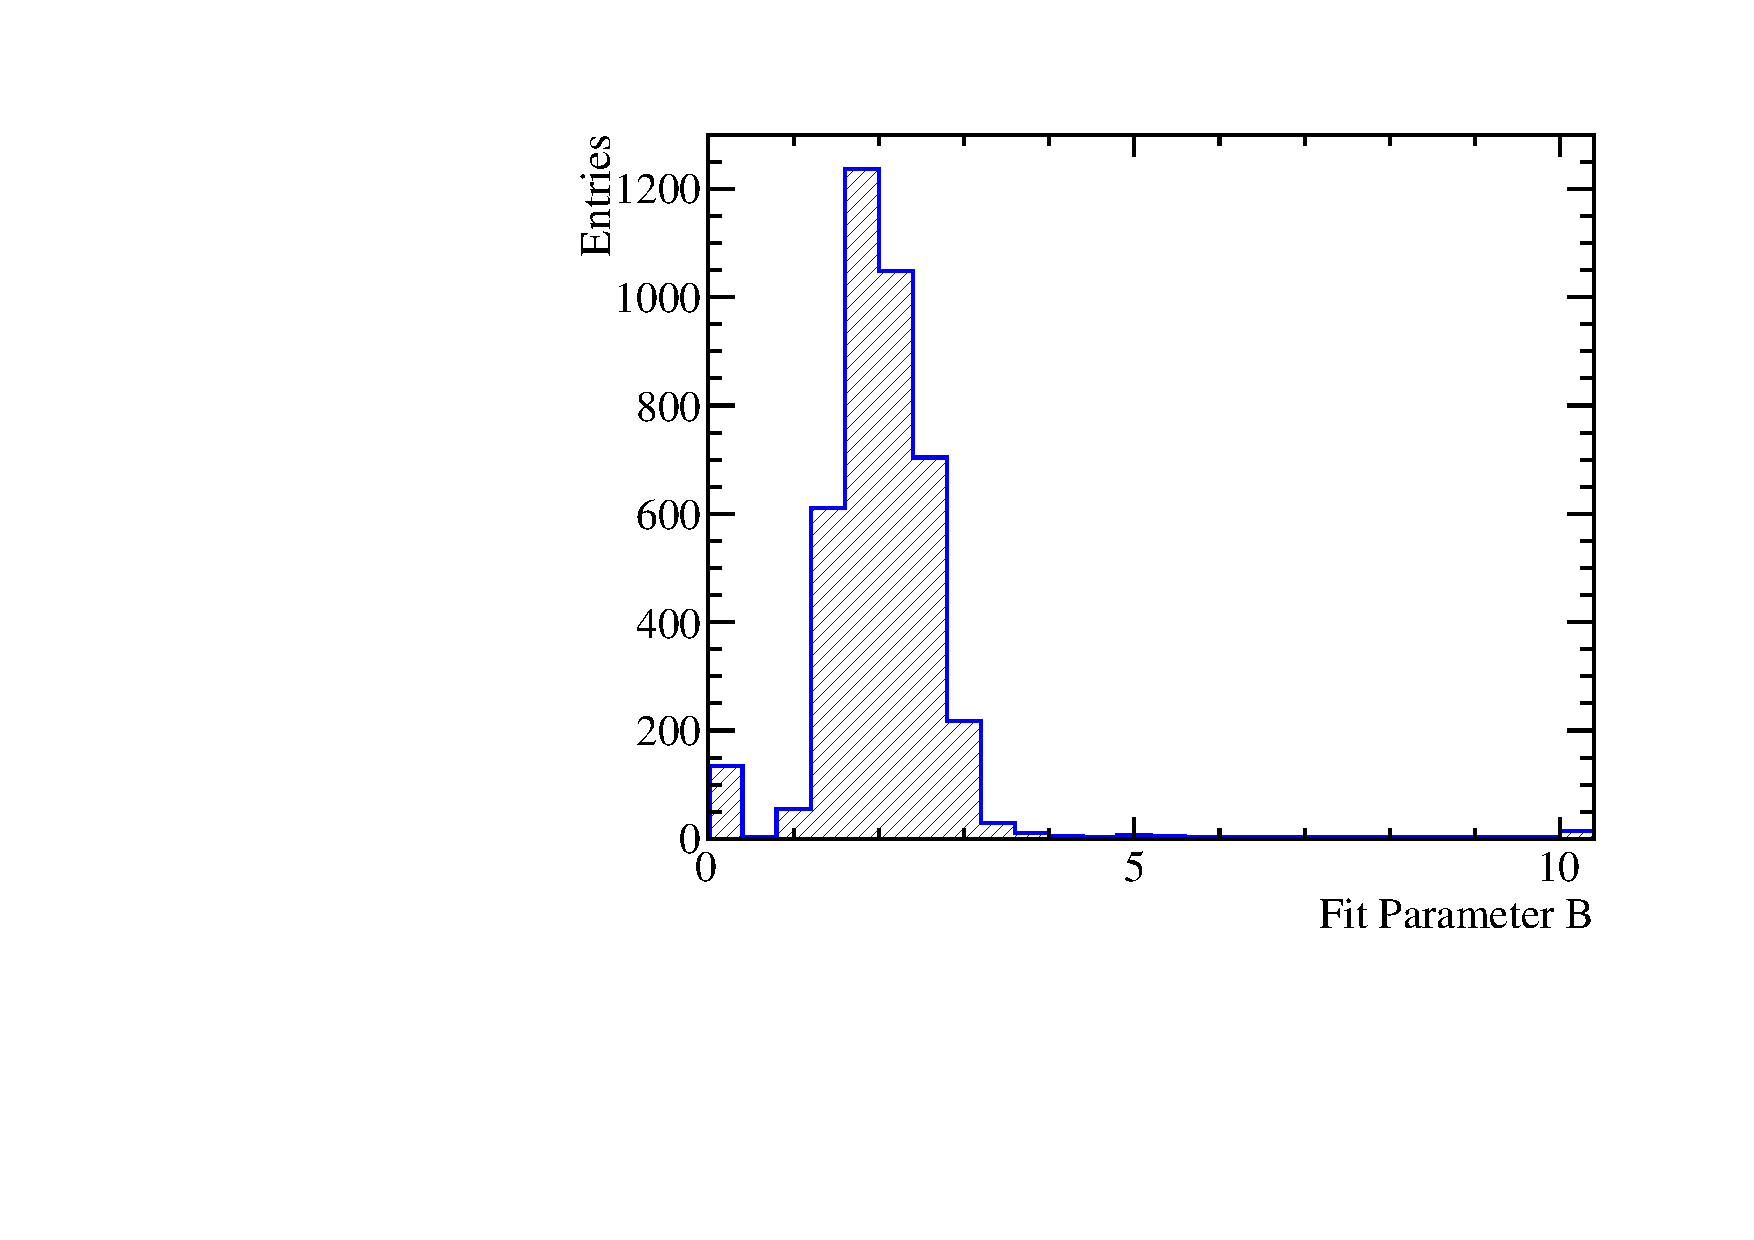
\includegraphics[width=0.5\textwidth]{CLICdpVertex/Plots/TestPulseCalibration/FitParam/OneDHistFitParamB_Set9.pdf}}\hfill
\subfloat[$c$ parameter.]{\label{fig:fitparams3}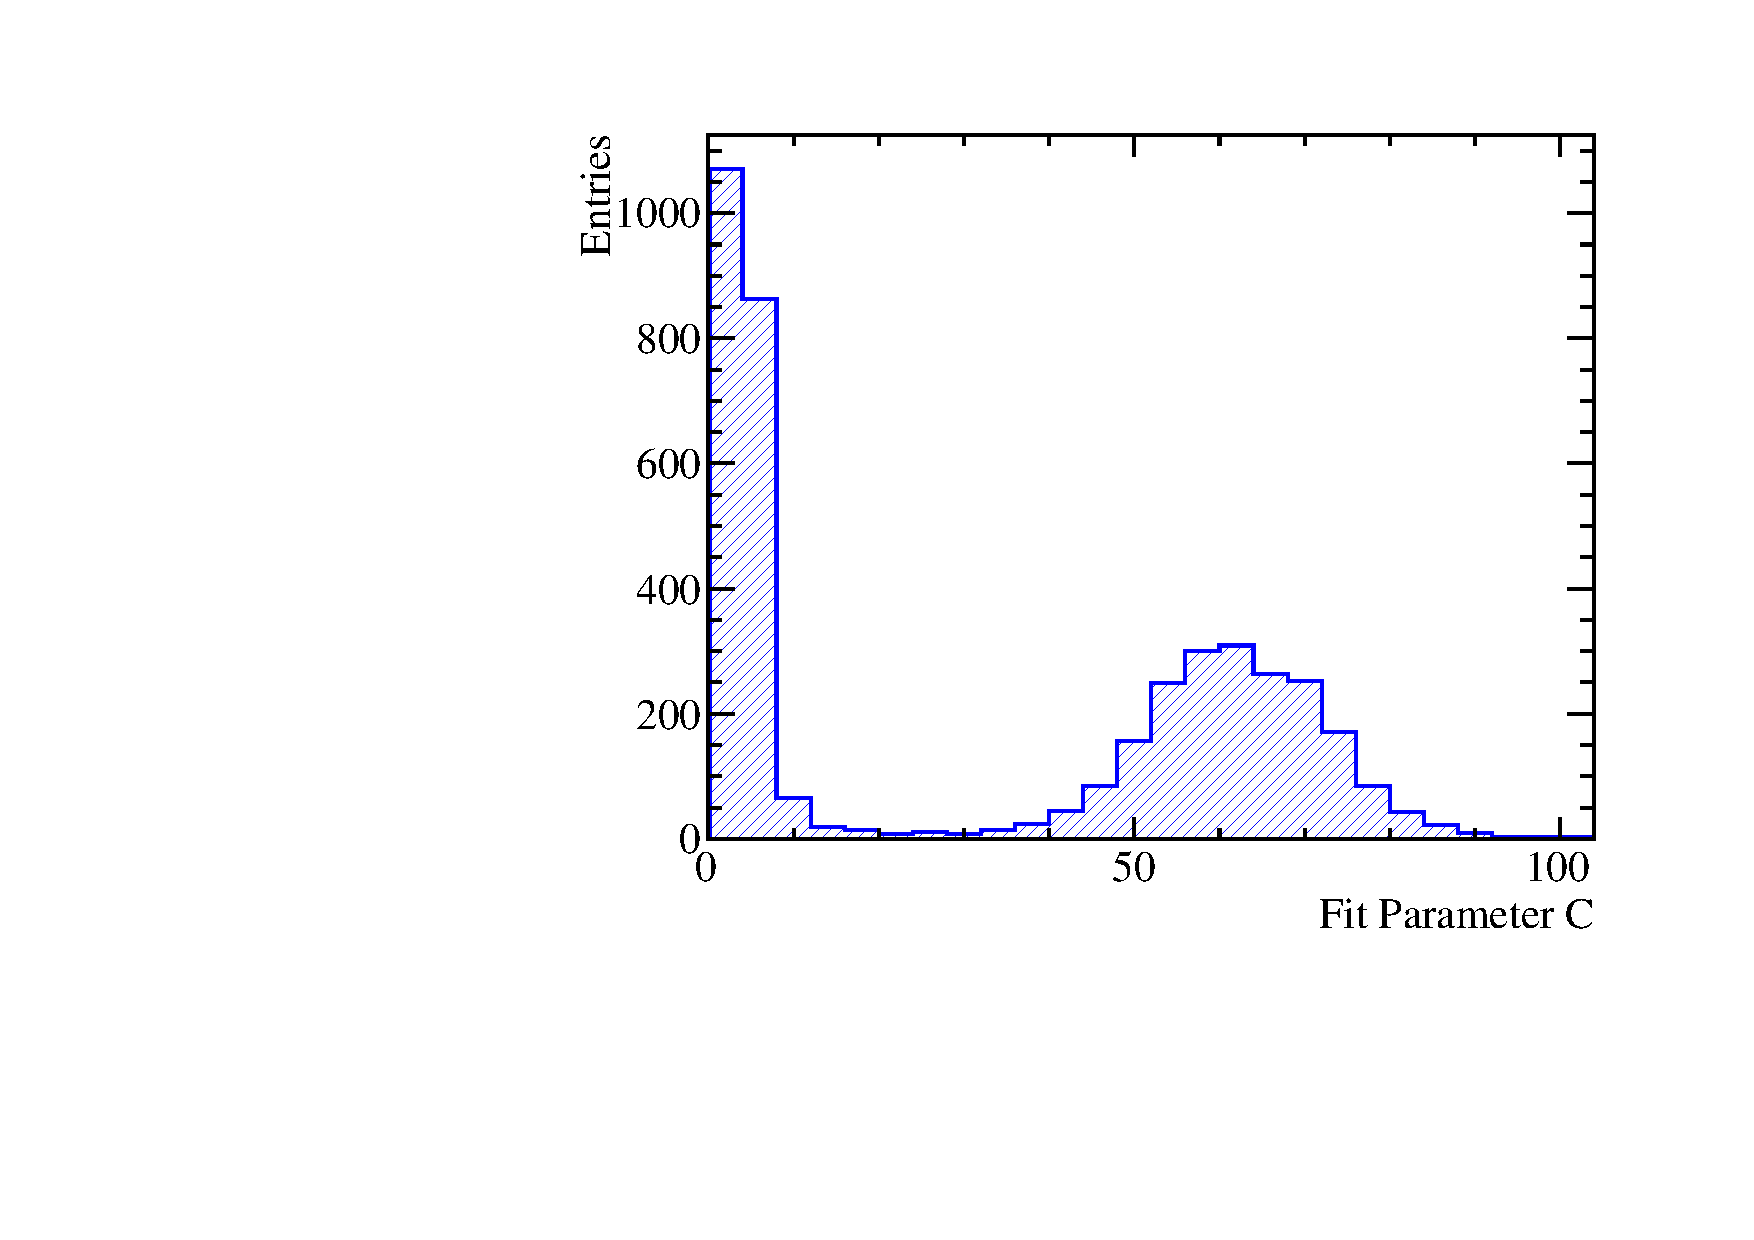
\includegraphics[width=0.5\textwidth]{CLICdpVertex/Plots/TestPulseCalibration/FitParam/OneDHistFitParamC_Set9.pdf}}
\subfloat[$t$ parameter.]{\label{fig:fitparams4}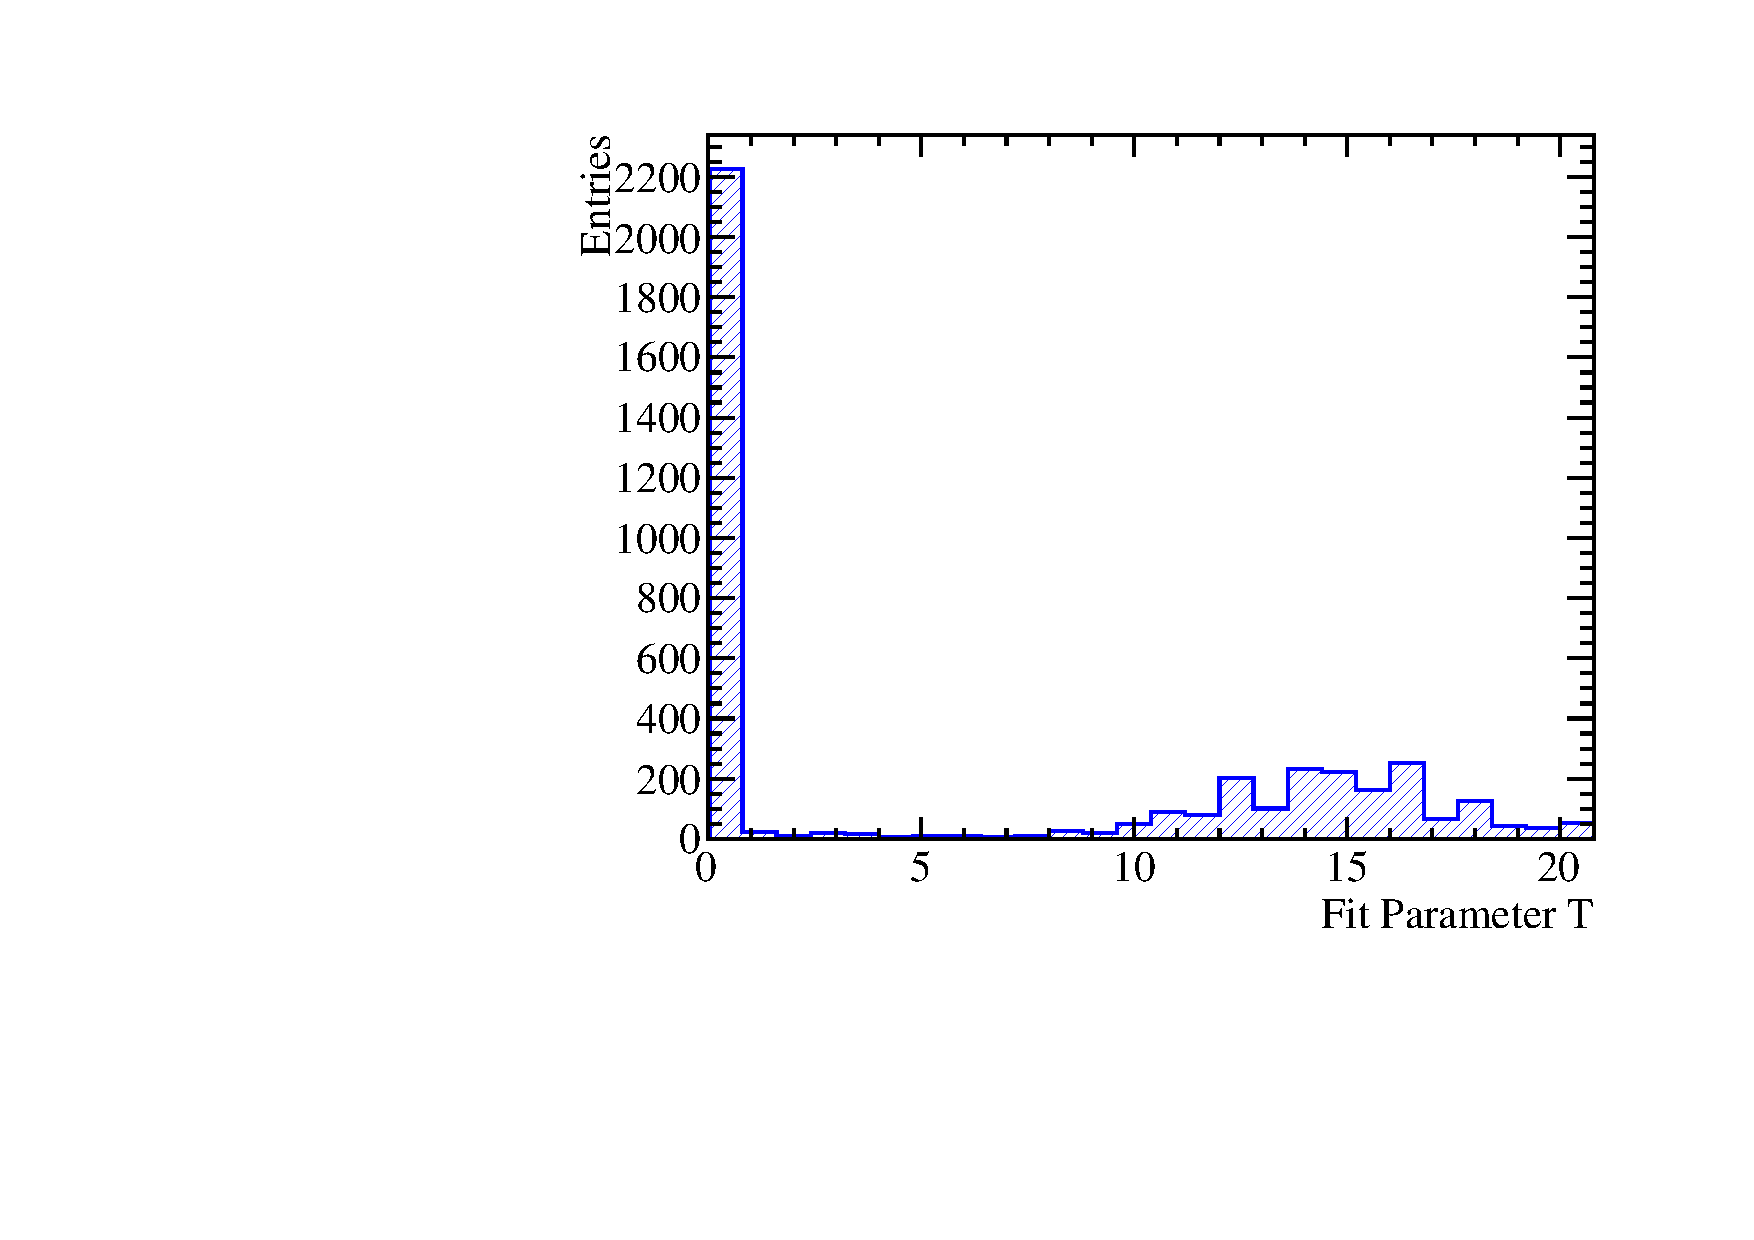
\includegraphics[width=0.5\textwidth]{CLICdpVertex/Plots/TestPulseCalibration/FitParam/OneDHistFitParamT_Set9.pdf}}
\label{fig:fitparams}
\caption[Distribution of surrogate function fit parameters for Set 9.]{Distribution of surrogate function fit parameters for Set 9.}
\end{figure}

\begin{figure}
\centering
\subfloat[$c$ parameter.]{\label{fig:fitparams2dc}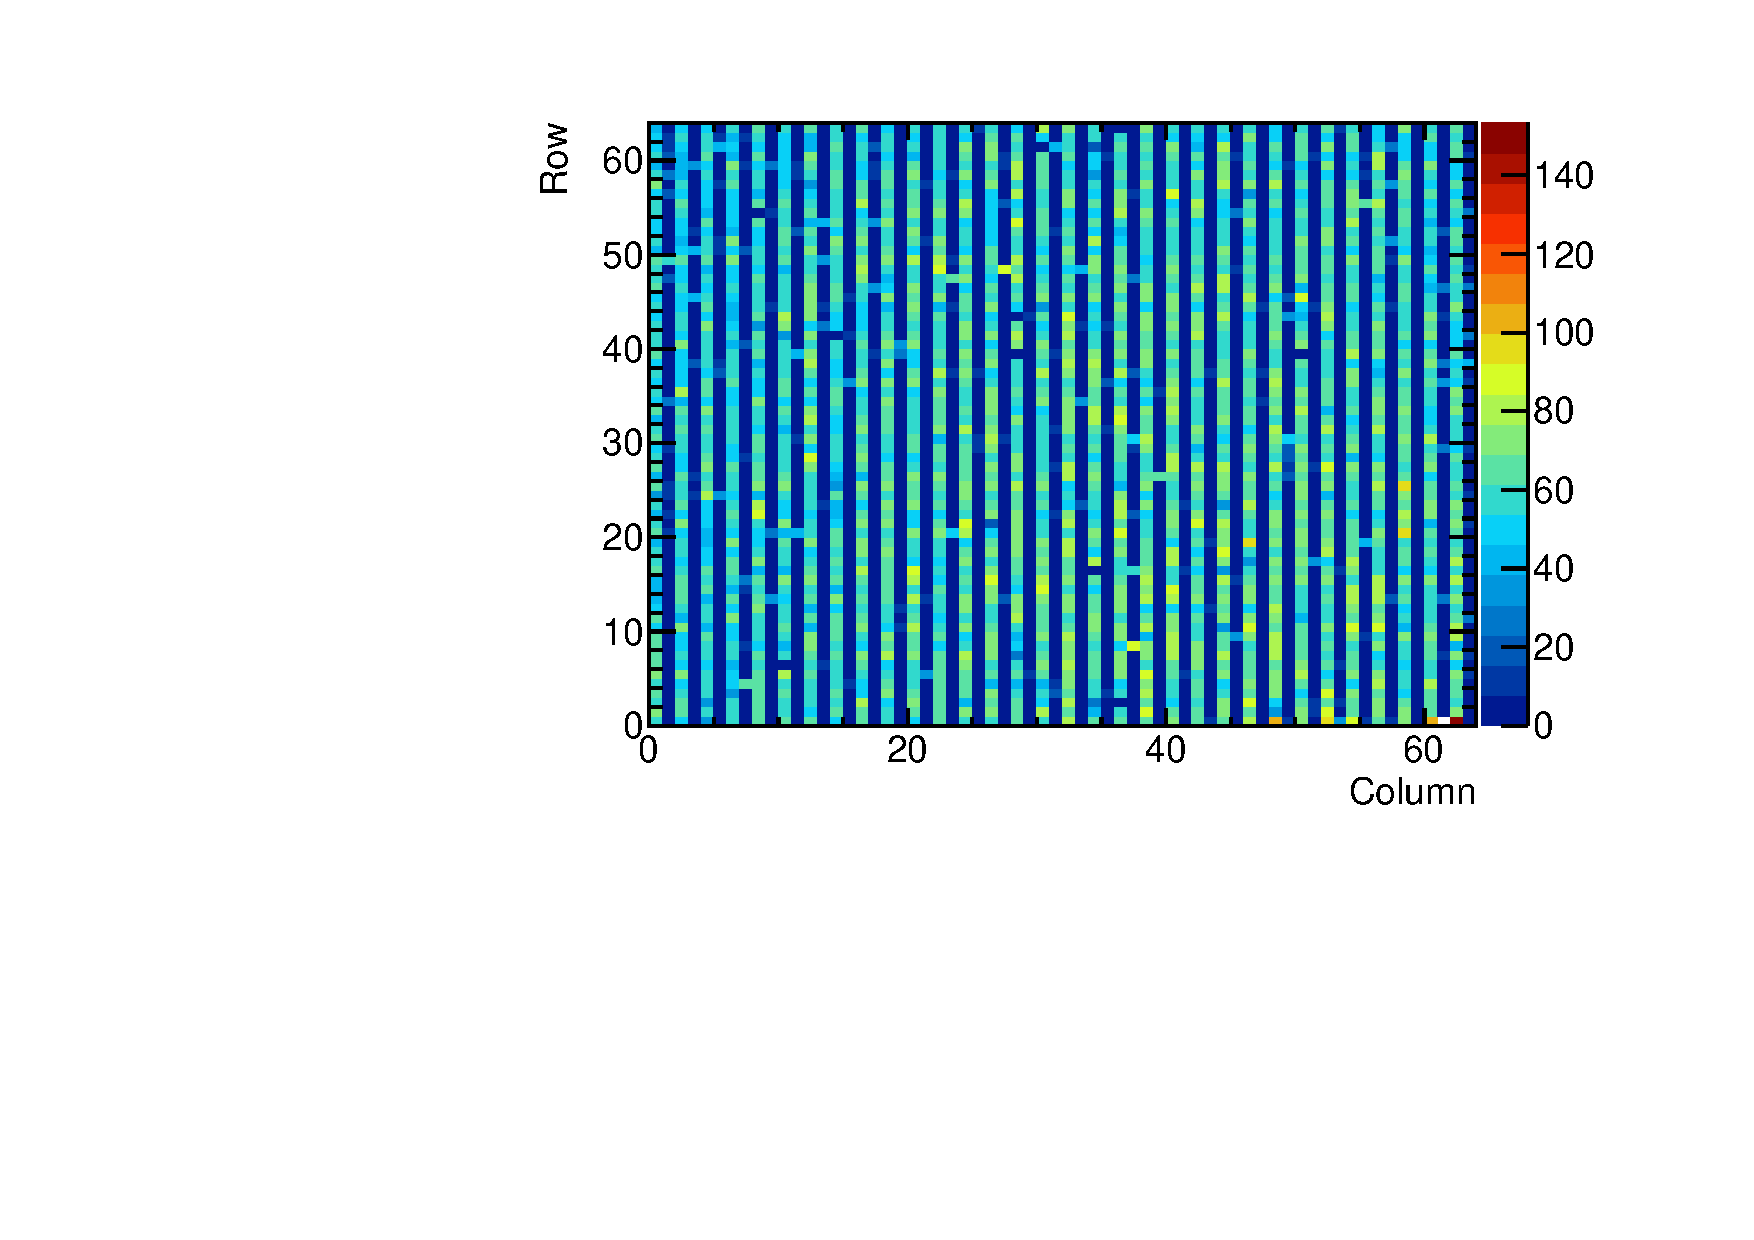
\includegraphics[width=0.5\textwidth]{CLICdpVertex/Plots/TestPulseCalibration/FitParam/FitParamC_Set9.pdf}}
\subfloat[$t$ parameter.]{\label{fig:fitparams2dt}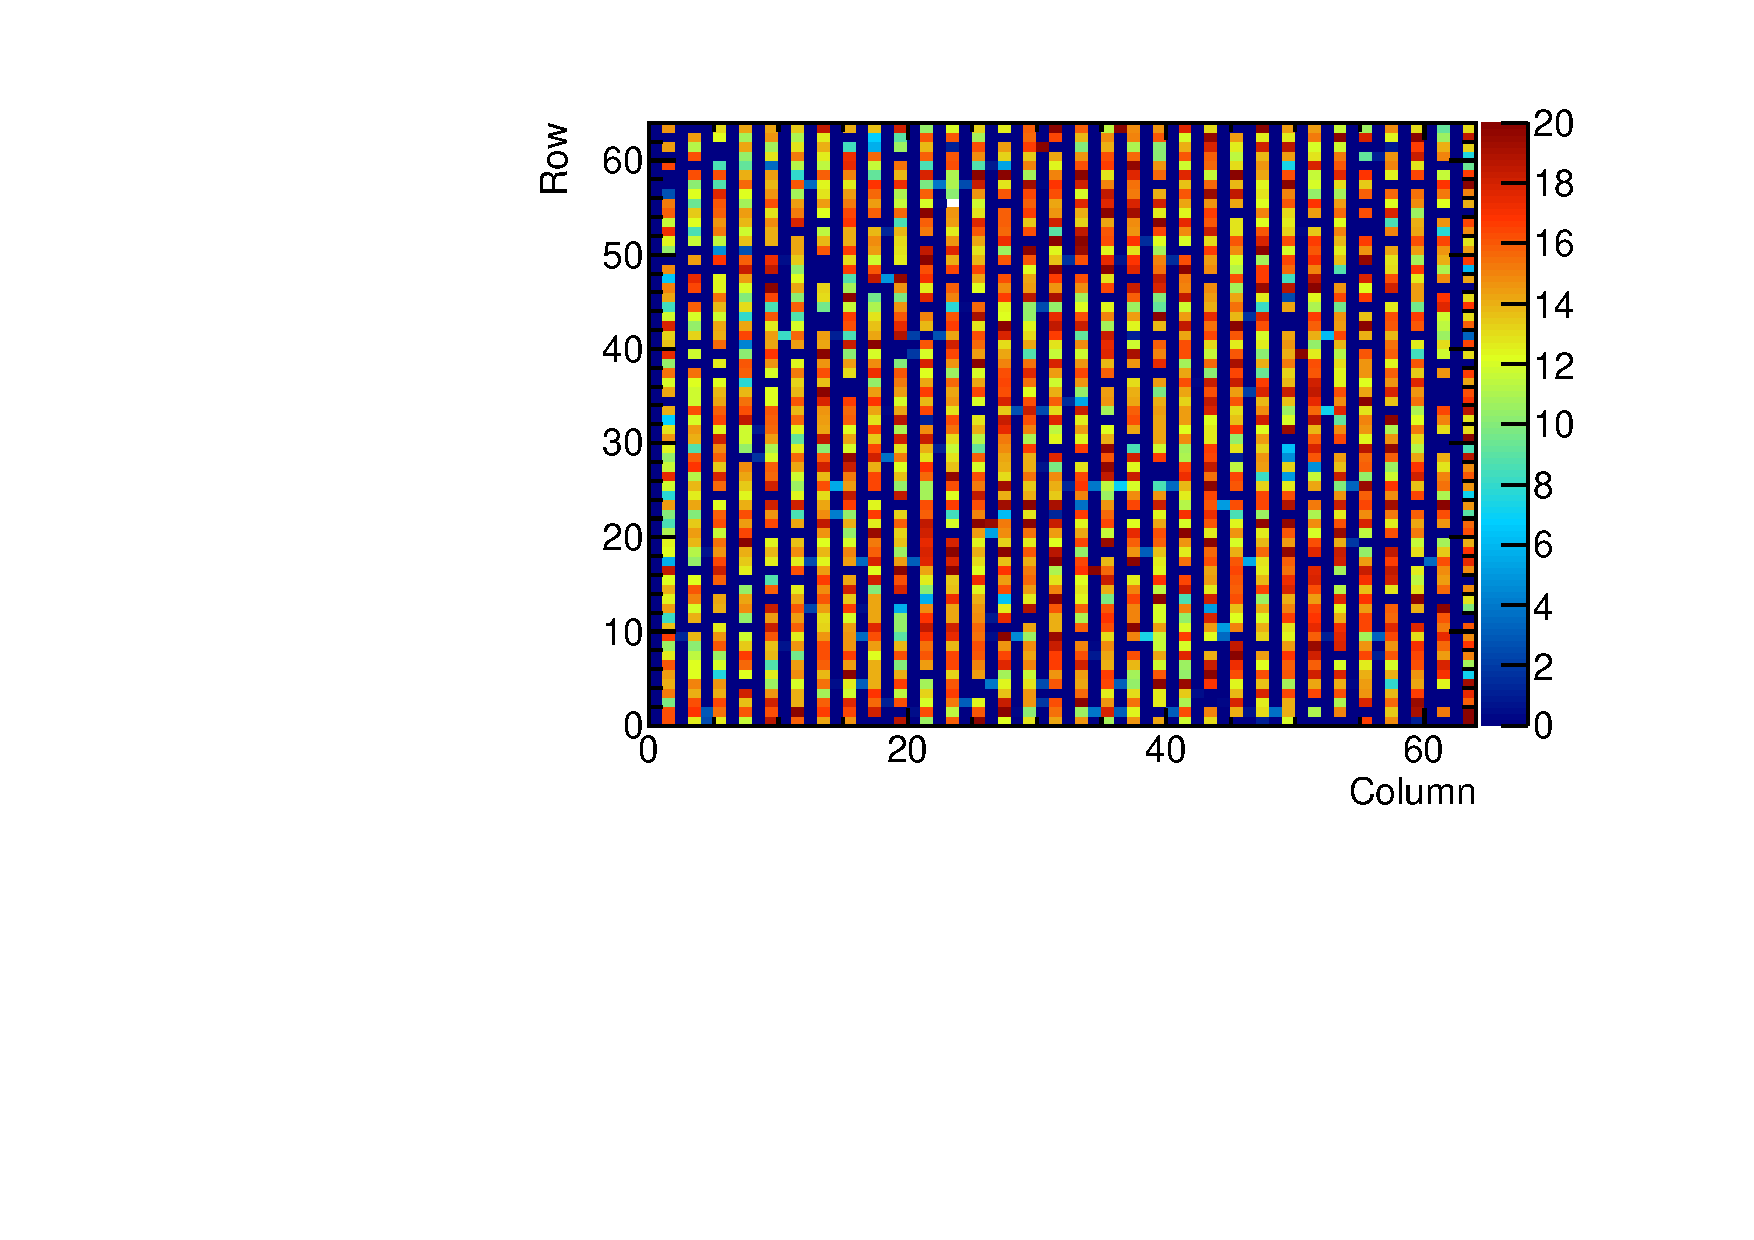
\includegraphics[width=0.5\textwidth]{CLICdpVertex/Plots/TestPulseCalibration/FitParam/FitParamT_Set9.pdf}}
\label{fig:fitparams2d}
\caption[Distribution as a function of matrix position of surrogate function fit parameter $c$ for Set 9.]{Distribution of surrogate function fit parameters $c$ and $t$ for Set 9.}
\end{figure}

The average of the surrogate function fit parameters for all devices considered can be found in table \ref{table:clicpixfitparamseven} and  \ref{table:clicpixfitparamsodd} for the even and odd columns respectively.  The surrogate function using these average parameters as input is shown in figure \ref{fig:testpulsemeanfit}.

\begin{table}[h!]
\centering
\begin{tabular}{ l r r r r}
\hline
Assembly & $a$ & $b$ & $c$ & $t$ \\ 
\hline
SET 9   & $0.0875 \pm 0.0005$ & $2.41 \pm 0.03$ & $5.1 \pm 0.1$ & $12.79 \pm 0.15$ \\
SET 10 & $0.0769 \pm 0.0005$ & $2.58 \pm 0.03$ & $7.5 \pm 0.2$ & $8.02 \pm 0.14$ \\
SET 12 & $0.0725 \pm 0.0005$ & $2.87 \pm 0.04$ & $12.1 \pm 0.3$ & $7.86 \pm 0.22$  \\
SET 13 & $0.0708 \pm 0.0005$ & $2.69 \pm 0.03$ & $16.2 \pm 0.3$ & $6.65 \pm 0.18$ \\
SET 14 & $0.0748 \pm 0.0005$ & $2.57 \pm 0.04$ & $16.0 \pm 1.3$ & $9.89 \pm 0.28$ \\
SET 15 & $0.0856 \pm 0.0005$ & $2.34 \pm 0.03$ & $5.1 \pm 0.2$ & $12.51 \pm 0.13$ \\
SET 16 & $0.0746 \pm 0.0004$ & $2.32 \pm 0.02$ & $13.7 \pm 0.3$ & $6.65\pm 0.16$ \\
\hline
\end{tabular}
\caption[Average fit parameters for even columns of CLICpix sensor.]{Average fit parameters for even columns of CLICpix sensor.}
\label{table:clicpixfitparamseven}
\end{table}

\begin{table}[h!]
\centering
\begin{tabular}{ l r r r r}
\hline
Assembly & $a$ & $b$ & $c$ & $t$ \\ 
\hline
SET 9   & $0.0834 \pm 0.0003$ & $1.72 \pm 0.01$ & $61.0 \pm 0.3$ & $0.25 \pm 0.09$ \\
SET 10 & $0.0759 \pm 0.0002$ & $1.63 \pm 0.01$ & $43.2 \pm 0.2$ & $0.10 \pm 0.02$ \\
SET 12 & $0.0731 \pm 0.0003$ & $1.92 \pm 0.02$ & $51.5 \pm 0.3$ & $0.36 \pm 0.12$ \\
SET 13 & $0.0713 \pm 0.0002$ & $1.72 \pm 0.01$ & $52.5 \pm 0.3$ & $0.18 \pm 0.07$ \\
SET 14 & $0.0754 \pm 0.0002$ & $1.68 \pm 0.01$ & $57.3 \pm 0.3$ & $0.16 \pm 0.03$ \\
SET 15 & $0.0836 \pm 0.0003$ & $1.52 \pm 0.02$ & $52.7 \pm 0.3$ & $0.42 \pm 0.08$ \\
SET16  & $0.0727 \pm 0.0002$ & $1.49 \pm 0.01$ & $50.7 \pm 0.2$ & $0.10 \pm 0.03$ \\
\hline
\end{tabular}
\caption[Average fit parameters for odd columns of CLICpix sensor.]{Average fit parameters for odd columns of CLICpix sensor.}
\label{table:clicpixfitparamsodd}
\end{table}

\begin{figure}
\centering
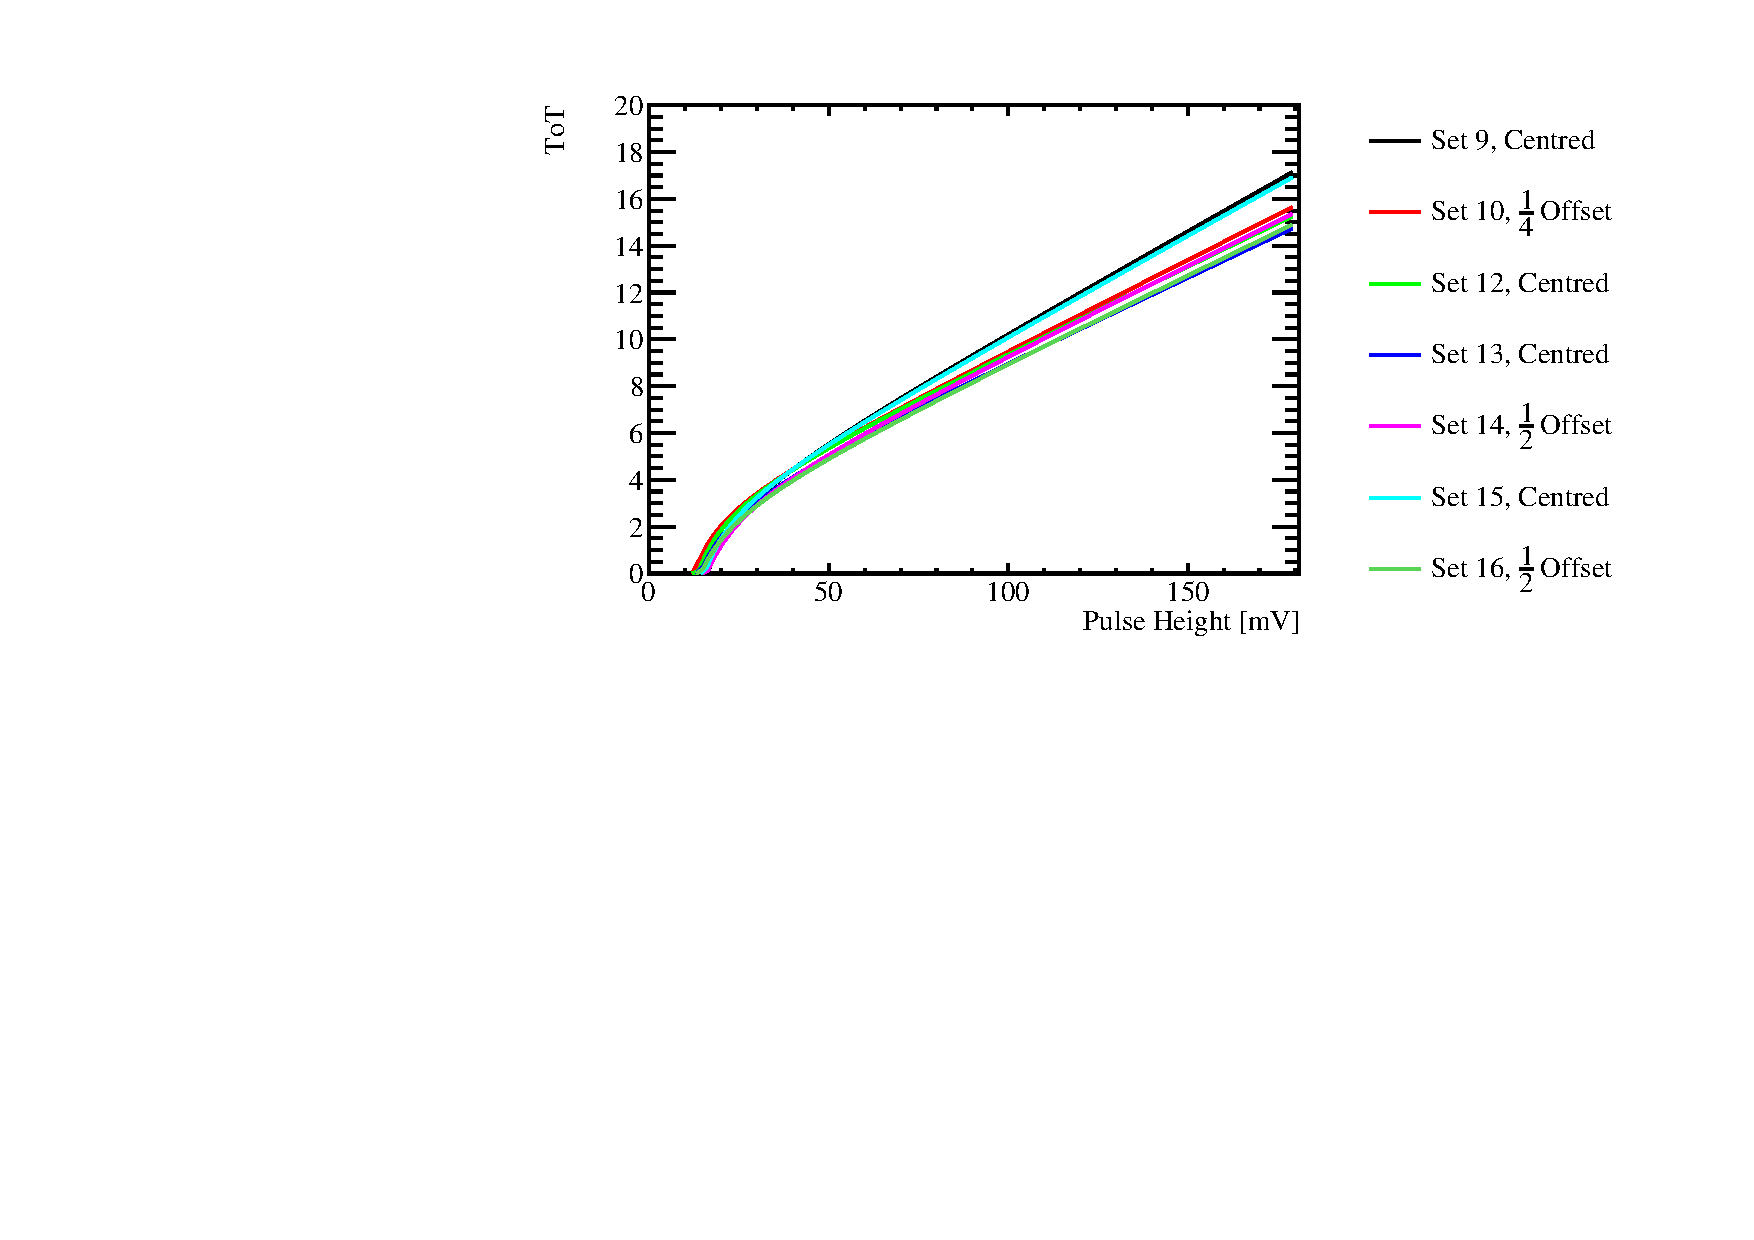
\includegraphics[width=1.0\textwidth]{CLICdpVertex/Plots/TestPulseCalibration/FitParam/AverageToT_vs_InjectedPulseHeight.pdf}
\caption[Fitted CLICpix ToT as a function of injected pulse height averaged across the device matrix.]{Fitted CLICpix ToT as a function of injected pulse height averaged across the device matrix.}
\label{fig:testpulsemeanfit}
\end{figure}

As figure \ref{fig:testpulsemeanfit} shows the response of the CLICpix to the injected pulse height is rather uniform across all samples considered.  In general, the turn on pulse height is $\approx$ 10 mV and saturation (i.e. ToT of 15 units) occurs at $\approx$ 150 mV.  For even numbered columns there is a sharper rise in ToT than for odd numbered columns due to the different effective threshold effect that is present in the CLICpix sensor.  This effect was observed across all devices considered.  In summary, this data presents a strong indication that the behaviour of the CLICpix ASIC is not affected by the presence of the HV-CMOS device either with or without an offset.  Therefore, performance changes between these sensors is entirely due to the HV-CMOS and the transmission of the signal it produces to the CLICpix.  

%========================================================================================
%========================================================================================

\section{Test Beam Analysis}
\label{sec:testbeam}
This sections describes the performance of the devices when placed under real experimental conditions at the CERN test beam area.  

%========================================================================================

\subsection{Test Beam Setup}
The overall goal of this experiment was to determine the tracking performance of the capacitively coupled pixel sensors and to see whether the misalignment of the HV-CMOS and the CLICpix changes the performance.  To that end the samples were mounted on a telescope and placed in a test beam to determine the efficiency, defined as the ratio of number of recorded tracks passing through device to the actual number of tracks passing through device, of the samples.  

These test beam experiments were carried out in August and September 2015 on the H6 beam line in the CERN SPS North Area.  The beam consisted of positively charged hadrons of momenta 120 GeV/c.  Mean particle rates of 500 kHz/cm$^{2}$ were observed during the 4.8 s spills at intervals of 25 s.  \textcolor{red}{Is this data correct?}.

During this experiment the samples mounted on an EUDET/AIDA telescope \cite{Rubinskiy:2000287}, which consists of six planes sensors using the Mimosa pixel technology.  This telescope provides a resolution of 1.6 $\mu$m on the intercept position between tracks passing through the device and the device under test (DUT) mounted on it.  

%========================================================================================

\subsection{Analysis}
The track position on the DUT was estimated by extrapolation based on the telescope sensor data.  This was followed by a search around the intercept position on the DUT to find clusters of hits.  The scan covered a region of 75 $\mu$m, or 3 pixels, about the intercept position.  For any multi-pixel clusters the ToT weighted centre of gravity was used to determine the position.  Several tracks during this experiment undergo scattering making them unsuitable for this analysis and these tracks were vetoed using a $\chi^{2}$ cut.  Some pixels on the device were deemed to be noisy and so were vetoed from the analysis along with any tracks occurring within half a pixel of them.  A pixel was deemed noisy if it responded at a mean rate \textcolor{red}{Clarify} greater than 5 $\sigma$ in comparison to the average rate.  Finally all tracks occurring within 125 $\mu$m of each other were vetoed.  \textcolor{red}{Is this data correct, taken from previous cern note?}

An alignment procedure is applied to both the telescope sensor planes as well as the DUT.  The six telescope sensor planes were aligned sequentially by minimising $\chi^{2}$, the distance between a cluster in a given plane and the intercept of an associated track divided by the \textcolor{red}{Error?}, as a function of the orientation of a given plane.  After the sensor planes were aligned the DUT was aligned by minimising the quadrature sum of the residuals, the difference between the cluster centre on the DUT and the associated track intercept.  

%========================================================================================

\subsection{Efficiency}
The efficiency, $\epsilon$, is defined as the number of tracks recorded by the CLICpix sensor, $n$, divided by the number of tracks passing through the device according the the telescope data, $m$.  This experiment is governed by binomial statistics as every track that passes through the telescope either is or is not recorded by the CLICpix.  The errors shown on the efficiency measurements are given by $\sqrt{\frac{\epsilon (1 - \epsilon)}{m}}$, which follows from the variance of $n$ given binomial statistics with mean $\epsilon$.  

\begin{figure}
\centering
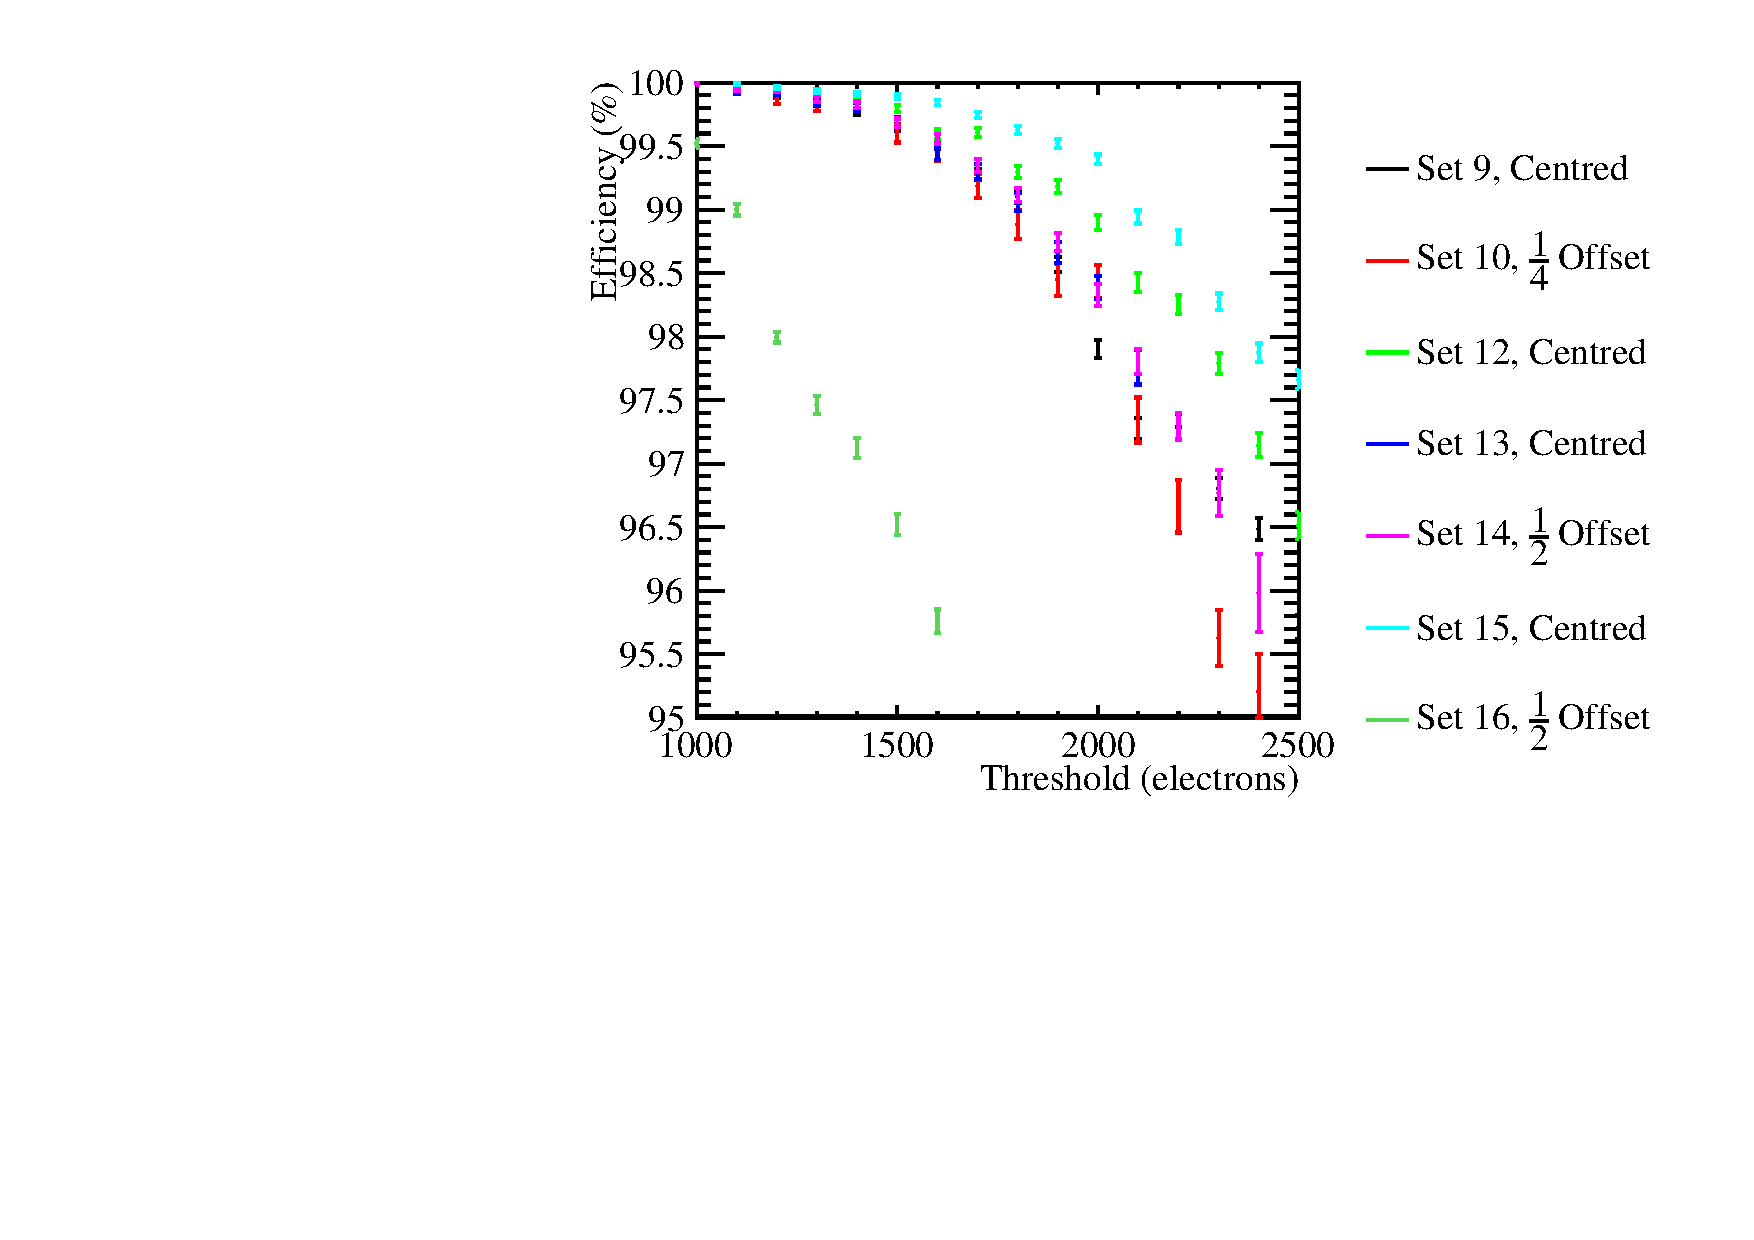
\includegraphics[width=1.0\textwidth]{CLICdpVertex/Plots/TestBeamData/EfficiencyThresholdPlot.pdf}
\caption[Efficiency as a function of threshold.]{Efficiency as a function of threshold.}
\label{fig:efficiency}
\end{figure}

The efficiency as a function of threshold used for the ToT calculation is shown in figure \ref{fig:efficiency}.  This data indicates that, as expected, for all sensors the efficiency of the sensor registering tracks decreases when increasing the number of electrons required to generate the signal.  However, it is clear that for the $\frac{1}{2}$ offset sample, Set 16, the efficiency is significantly lower in comparison to the other samples.  Again, the remaining $\frac{1}{2}$ offset sample, Set 14, behaves as a centred sample indicating a mistake in the manufacturing procedure.  There is a minor degradation in performance when considering the $\frac{1}{4}$ offset sample, but these results are still comparable to several of the centred samples.  Overall, it can be concluded that manufacturing tolerances up to $\frac{1}{4}$ of a pixel width would not significantly affect performance.    

%========================================================================================

\section{Conclusions}


%========================================================================================

  
